\documentclass[12pt]{book}
\usepackage[utf8]{inputenc}
\usepackage[spanish,es-tabla]{babel}
\usepackage[table]{xcolor}
\usepackage{amsmath}
\usepackage{amsfonts}
\usepackage{graphicx}
\usepackage{xcolor}
\usepackage{subfigure}
\usepackage{tikz}
\usepackage{cleveref}
\usepackage{microtype}
\usepackage{geometry}
\usetikzlibrary{calc}
\usetikzlibrary{circuits}
\renewcommand{\arraystretch}{1.5}
\renewcommand{\baselinestretch}{1.5}
\title{TFG}
\author{Francisco Gómez Prieto}
\usepackage{amssymb}
\usepackage{theorem}
\usepackage{color}
\usepackage{amscd}
%\usepackage{showidx}
\usepackage{textcomp}
\usepackage{pdfpages}
\usepackage{afterpage}
\usepackage{makeidx}
\usepackage{graphicx}
\usepackage{caption}
\usepackage{float}
\usepackage{wrapfig}
\usepackage{listings}
\usepackage{multicol}
\usepackage{cite}
\usepackage[toc,page]{appendix}

\renewcommand{\appendixtocname}{Ap\'endices}
\renewcommand{\appendixpagename}{Ap\'endices}

%PARA ESCRIBIR EL SÍMBOLO DEL EURO.
%\def\eu{\,\hbox{\raise .36em\hbox to0pt{\vrule height0.5pt%
%width.55em depth0pt\hss}%
%\raise .25em\hbox to0pt{\vrule height0.5pt width.5em%
%depth0pt\hss}\hskip.02em\sf C}\,}

% Imprime la fecha de revisión y la etiqueta
% 'Draft Version' (From Josullvn, CS, CMU)
%%%%%%%%%%%%%%%%%%%%%%%%%%%%%%%%%%%%%%%%%%%%
%\newcommand{\reviewtimetoday}[2]{\special{
%!userdict begin /bop-hook{gsave 20 710
%translate 45 rotate 0.8 setgray
%/Times-Roman findfont 12 scalefont setfont
%0 0 moveto (#1) show 0 -12 moveto (#2) show grestore}def end}}
%\reviewtimetoday{\today}{Draft Version}

\setlength{\textheight}{21cm} \setlength{\topmargin}{-.5cm}
\setlength{\footskip}{2cm}
\setlength{\oddsidemargin}{1.5cm}
\setlength{\evensidemargin}{-0.25cm}
\setlength{\textwidth}{15cm}

%\usepackage{fancyhdr}
%\pagestyle{fancy}
%\fancyhf{}
%\fancyhead[RE]{\MakeUppercase{CAP.\, \thechapter}}
%\fancyhead[LO]{}
%\fancyhead[RO,LE]{\bfseries \thepage}
%\fancyhead[CE]{\leftmark}
%\fancyhead[CO]{\rightmark}

%\renewcommand{\chaptermark}[1]{\markboth{\MakeUppercase{#1}}{}}
%\renewcommand{\chaptermark}[1]{\markboth{\chaptername\, \thechapter. #1}{}}
\renewcommand{\sectionmark}[1]{\markright{\thesection. #1}}
%\renewcommand{\headrulewidth}{.6pt}
%\renewcommand{\headrule}{\setlength=15cm}


\setlength{\headheight}{2.5\headheight}
%\renewcommand{\headrule}{\leftskip=.5cm}
%\fancyfoot{}
%\renewcommand{\headrule}{\vbox to 0pt{\hbox to 50pt}}
%\renewcommand{\headrule}{%
%\makebox[0pt][0]{\rule[3\baselineskip]{\linewidth}{0.8pt}}%
%\color[named]{Red}%
%\rule[-.3\baselineskip]{\linewidth}{0.4pt}}

% Limpia el encabezado en las páginas impares vacías
\makeatletter \def\cleardoublepage{
\clearpage\if@twoside \ifodd\c@page\else%
\hbox{}%
\thispagestyle{empty}% Aquí elimina el estilo del encabezado
\newpage%
\if@twocolumn\hbox{}\newpage\fi\fi\fi} \makeatother

\providecommand{\norm}[1]{\lVert#1\rVert}

%\usepackage[active]{srcltx}


\def\blacksquare{\hbox{\vrule width 4pt height 4pt depth 0pt}}
\def\qed{\ \ \ \hbox{}\nolinebreak\hfill $\blacksquare \  \  \  \  $ \par{}\medskip}


\newtheorem{theorem}{Teorema}[section]
\newtheorem{teorema}[theorem]{Teorema}
\newtheorem{lemma}[theorem]{Lema}
\newtheorem{proposicion}[theorem]{Proposición}
\newtheorem{corolario}[theorem]{Corolario}




\newtheorem{ejemplo}[theorem]{Ejemplo}
\newtheorem{definicion}[theorem]{Definición}
\newtheorem{ejercicio}[theorem]{Ejercicio}
\newtheorem{notacion}[theorem]{Notación}


\newtheorem{observacion}[theorem]{Observación}

\numberwithin{equation}{section}


\newcommand{\teor}{\begin{teorema}}
\newcommand{\eteor}{\end{teorema}}
\newcommand{\prop}{\begin{proposicion}}
\newcommand{\eprop}{\end{proposicion}}
\newcommand{\coro}{\begin{corolario}}
\newcommand{\ecoro}{\end{corolario}}
\newcommand{\lema}{\begin{lemma}}
\newcommand{\elema}{\end{lemma}}
\newcommand{\ejer}{\begin{ejercicio}}
\newcommand{\eejer}{\end{ejercicio}}
\newcommand{\obse}{\begin{observacion}}
\newcommand{\eobse}{\end{observacion}}
\newcommand{\defi}{\begin{definicion}}
\newcommand{\edefi}{\end{definicion}}
\newcommand{\demo}{\begin{proof}[Demostración]}
\newcommand{\edemo}{\end{proof}}
\newcommand{\ejem}{\begin{ejemplo}}
\newcommand{\eejem}{\end{ejemplo}}
\newcommand{\nota}{\begin{notacion}}
\newcommand{\enota}{\end{notacion}}
\newcommand{\nada}{\begin{naida}}
\newcommand{\enada}{\end{naida}}
\newcommand{\vaci}{\begin{vacio}}
\newcommand{\evaci}{\end{vacio}}
\newcommand{\sucesion}{(x_n)_{n\in \mathbb{N}}}
\newcommand{\sucesionpelada}{(x_n)}
\usepackage[all]{xypic}

%\newenvironment{flushenum}{  %%% NO INDENTA LOS ITEMS EN UNA ENUMERACIÓN
%\begin{enumerate}            %%%
%  \setlength{\leftmargin}{0pt}%%%
%}{\end{enumerate}}            %%%



\usepackage{enumitem}  
%PERMITE, POR EJEMPLO, QUITAR "INDENTS" DE LOS "ITEMS" (Poniendo %%%%%%%%%%%%%%%%%%%%%%%%\begin{enumerate}[leftmargin=*] %+y, luego, todo igual %que siempre.)

%\includegraphics


\renewcommand{\listtablename}{Índice de tablas}
\renewcommand{\tablename}{Tabla} 

\usepackage[final]{epsfig}
\date{}
\makeindex

\begin{document}
\pagestyle{empty}
\lstset{language=Java, columns=flexible}
\includepdf[pages={8}]{./normativa3.pdf}

\newpage
~

\newpage
Fernando Javier Álvarez Franco, profesor del departamento de Ingeniería Eléctrica, Electrónica y Automática de la universidad de Extremadura.

INFORMA:

Que D. Francisco Gómez Prieto ha realizado bajo su dirección el Trabajo de Fin de Grado. Considera que la memoria reúne los requisitos necesarios para su evaluación.

\medskip

\begin{flushright}
Badajoz, 26 de Junio de 2019
\end{flushright}

\vspace{8\baselineskip}
\begin{center}
Fdo. Fernando Javier Álvarez Franco.
\end{center}
\newpage
~
\newpage
\setcounter{page}{1}
\pagestyle{plain}
\tableofcontents

\newpage
~

\newpage
\chapter*{Resumen}
\addcontentsline{toc}{chapter}{Resumen}
El objetivo de este trabajo fin de grado es estudiar dónde se encuentra la tecnología de identificación de patrones motores y realizar una aplicación práctica sobre la detección del tipo de movimiento centrándonos en cuatro tipos: Estacionario, corriendo, andando y caída.

Con este objetivo presente, se utilizaran los medios más actualizados para la realización del proyecto experimental, en este caso, las redes neuronales, una técnica de inteligencia artificial.-

Además, se usará un \textit{smartwatch} para realizar la toma de datos, tomando datos muchos más útiles para esta aplicación, ya que el \textit{smartwatch} está en una posición fija del usuario. Otro objetivo es el tener una interfaz sencilla e intuitiva, para que personas adultas o ancianas no tengan ningún tipo de problema al utilizar el sistema.


\newpage
\chapter*{Abstract}
\addcontentsline{toc}{chapter}{Abstract}


The objective of this work is study about the technology involving vital signal and create an app about movement patterns involving these four types of movements: Stationary, running, walking and falling down.

With that objective in mind, we will use the most advanced methods to do the experimental project, and neural networks and other algorithms of artificial intelligence are those advanced methods.

Also, we will use a \textit{smartwatch} as data retriever. This way we will obtain very precise data without draining the user's \textit{smartphone} battery. Another objective is having a simple and intuitive interface, so the elderly and adults alike don't have any problem using the system.

\newpage
\chapter{Introducción}

En este trabajo se pretende clasificar los tipos de movimientos mediante un dispositivo \textit{wearable} Android. Para ello se van a usar un \textit{smartphone} Android, un reloj con sistema operativo \textit{WearOS}, que es simplemente Android Wear actualizado.

Para la clasificación se va a usar un sistema de inteligencia artificial, basado en redes neuronales cuyo objetivo es ir identificando en tiempo real el tipo de movimiento y mostrar los resultados de esta clasificación en pantalla.

Este tipo de monitorización contínua es muy interesante ya que hay enfermedades en las que un estudio con seguimiento continuo puede ser usado para establecer el estado de la enfermedad en el usuario y a partir de esta información mejorar la calidad de vida de los pacientes.

Otra aplicación más comercial sería la detección de distintos tipos de ejercicio para una optimización del movimiento realizado por atletas profesionales o para amateurs, una simple aplicación de ejercicio para contar kilocalorias, que es una opción bastante demandada si nos fijamos en el número de Apps que hay en las \textit{stores} de Android y iOS.

La principal contribución de este trabajo es la implementación en \textit{WearOS}, permitiendo su uso en multitud de dispositivos y tomando datos mucho más útiles que si los tomara desde el \textit{smartphone}, ya que el reloj es un dispositivo situado en la muñeca, al contrario que los \textit{smartphones}. Esto es una ventaja pues permite ahorrar el trabajo de posicionar el dispositivo con respecto al cuerpo, pues está fijo, simplificando el código de forma considerable.
\chapter{Antecedentes}
A continuación, se va a hacer un recorrido histórico de la evolución de la tecnología usada, empezando por las redes neuronales y posteriormente los acelerómetros y los algoritmos de clasificación de movimiento.
\section{Inteligencia artificial: Redes neuronales}
A lo largo de la historia de la humanidad, esta ha soñado con crear máquinas que tuvieran inteligencia. Como todo, ya en la antigua Grecia se había mencionado el tema, con las leyendas de Hefesto, que creó varios autómatas para que le ayudaran en sus trabajos de herrería. Por  desgracia, aquella habilidad quedaba limitada a dioses por aquel entonces.

A lo largo de los siglos, se fue nutriendo esta rama de la ciencia, pero se puede decir que hasta mediados del siglo XX no hubo avances reales.

Las redes neuronales es un campo multidisciplinar en el que han trabajado informáticos, biólogos, médicos, físicos y matemáticos por nombrar solo algunos. Al ser una tecnología basada, vagamente, en la biología, no solo humana, sino también en felinos y otro tipo de mamíferos, en la estructura de nuestro cerebro, es imposible que hubiera habido un desarrollo previo a los descubrimientos de nuestro compatriota Santiago Ramón y Cajal.

\subsection{Primera ola (1949-1969)}

Se podría decir que la primera ola de investigación rigurosa en el campo comenzó cuando D.O. Hebb publicó su libro,\textit{The organization of behavior}, donde se propone la primera ley de aprendizaje, que sirvió como base para el entrenamiento de las primeras redes neuronales.

Durante esta época, se desarrollaron las primeras redes neuronales que resuelven problemas simples, inicialmente en circuitos electrónicos y posteriormente en simulaciones por ordenador, mucho más flexibles.

Estos resultados positivos hicieron que en el campo hubiera mucha investigación, y se produjeran grandes avances, como el algoritmo del Perceptrón, en 1957\cite{rosenblatt1957perceptron}. Este algoritmo aún hoy en día es la base del campo y sigue siendo un algoritmo útil, con pequeñas mejoras.

Durante esta época, había grandes esperanzas en el campo, aunque solo pudieran resolver los problemas más sencillos. Sin embargo, en 1969 Marvin Minsky publicó su libro, \textit{Perceptrons}\cite{minsky}. En él, con una rigurosa base matemática se exponen los límites a los que se enfrenta los algoritmos de la época y se enumeran diversos problemas sencillos que no pueden resolver las redes neuronales, como por ejemplo una simple puerta XOR. Minsky era un científico respetado y con prestigio, y la publicación de su libro hizo que la investigación y financiación del campo se redujera durante años.
\subsection{Segunda ola (1986-1995)}
Durante estos periodos iniciales, las publicaciones no fueron en revistas de prestigio científico, lo cual hizo que la información, además de reducirse, se esparciese, lo que provocó que el trabajo muchas veces no llegara entre investigadores del mismo campo.

Sin embargo, durante las dos olas, no se abandonó el trabajo, y debido a las limitaciones de potencia, se centró en dar una base teórica más rigurosa que la anterior.

En 1986 se publicó el algoritmo de retropropagación. Este algoritmo permitía el entrenamiento de múltiples capas en un perceptrón, permitiendo la resolución de problemas que el perceptrón original no podía resolver, que habían sido recopilados por Minsky en su libro. Este algoritmo, aunque publicado en 1986 por Rumelhart \textit{et al}\cite{Rumelhart:1988:LRB:65669.104451}, ya había sido descubierto y aplicado antes, pero como se comentó en los párrafos anteriores, la investigación estaba muy desperdigada en diversas revistas y no siempre llegaba a todos. Cabe mencionar en especial a Paul Werbos, que en 1974 en su tesis ya lo aplicó a redes neuronales\cite{werbos}. 

Este descubrimiento hizo que se revitalizara la investigación, solo en 1987 hubo cuatro congresos mundiales y más de 500 \textit{papers} sobre el tema.

Por otro lado, en Japón, se desarrolla el Cognitrón y el Neocognitrón. Estas redes están diseñadas tomando como objetivo la reproducción del funcionamiento de la vista en seres vivos, que con suma facilidad es capaz de reconocer miles de objetos y caras. Estos algoritmos no fueron muy usados en esta época, pues la simpleza del Perceptrón multicapa hacía que fuera mucho más usado. Sin embargo, con el paso de los años se empezó a apreciar las posibilidades de este tipo de red, siendo la piedra angular de lo que luego se han conocido como redes convolucionales, que son las más utilizadas actualmente.

Esta ola acabó a mediados de los 90, debido a varios factores. Primero, llevados por la emoción del momento, los investigadores sobreestimaron las capacidades de la tecnología, y cuando los objetivos que habían ofrecido a los inversores no se cumplieron, bajo la financiación del campo. Por otro lado, otras tecnologías de inteligencia artificial ofrecieron soluciones a problemas de la época. Esto hizo que la inversión fuera para esas otras tecnologías.

\subsection{Tercera ola (2007-?)}
Se podría decir que esta época fue un resurgimiento de la anterior pero con mucha mas potencia de cálculo.  Esto se debe a varios factores, el primero, el descubrimiento de algoritmos que reducían el tiempo de procesamiento en gran medida\cite{doi:10.1162/neco.2006.18.7.1527}. Estos algoritmos son fácilmente generalizables a muchos problemas, por lo que el proceso de entrenamiento de una red neuronal se hizo mucho más eficiente.


Esto hizo que se pudieran usar más datos de entrenamiento. La causa se debe a muchos factores, pero principalmente a la mejora de los sensores, que permite tomar muchos mas datos por segundo. También, gracias a estos métodos más eficientes, el mayor número de datos no afecta tanto al tiempo de entrenamiento de las redes.

Además, se empieza a aprovechar el otro tipo de hardware más especializado, como las tarjetas gráficas, que se utilizan para hacer el entrenamiento de estas redes neuronales, reduciendo aún más los tiempos de entrenamiento, ya que las tarjetas gráficas tienen una arquitectura ideal para realización de tareas matemáticas en paralelo.

Finalmente, pero no menos importante, esta tercera ola presenta muy buenos resultados, ganando concursos de clasificación y otras tareas más mundanas como pueden ser detección de caras, coches con conducción autónoma etc. Entre los concursos de clasificación, se mencionara en especial el ImageNet Large Scale Visual Recognition Challenge. En este concurso hay una colección de miles de imágenes, y pasó de un 26.1\% de error a un 15.3\%\cite{concursos} mediante una red neuronal convolucional en un año. Desde entonces, todo este tipo de concursos son ganados por redes de tipo CNN(\textit{Convoluted neural network}). Actualmente, el error está en torno al 3.0\%.

Estos descubrimientos y un enfoque más centrado en la profundidad de la red (número de capas de neuronas) hacen que a esta ola se la conozca como \textit{deep learning}. Este nombre quiere hacer hincapié en que son algoritmos de aprendizaje pero, al contrario que en otras épocas debido a limitaciones tecnológicas, con muchas capas de profundidad.

\subsection{Presente (2019)}

Actualmente, el \textit{deep learning} sigue siendo popular. Por ejemplo nos podemos guiar por un parámetro como las búsquedas de google en los últimos años, como muestra la figura \ref{fig:growth}.

\begin{figure}[h]
    \centering
    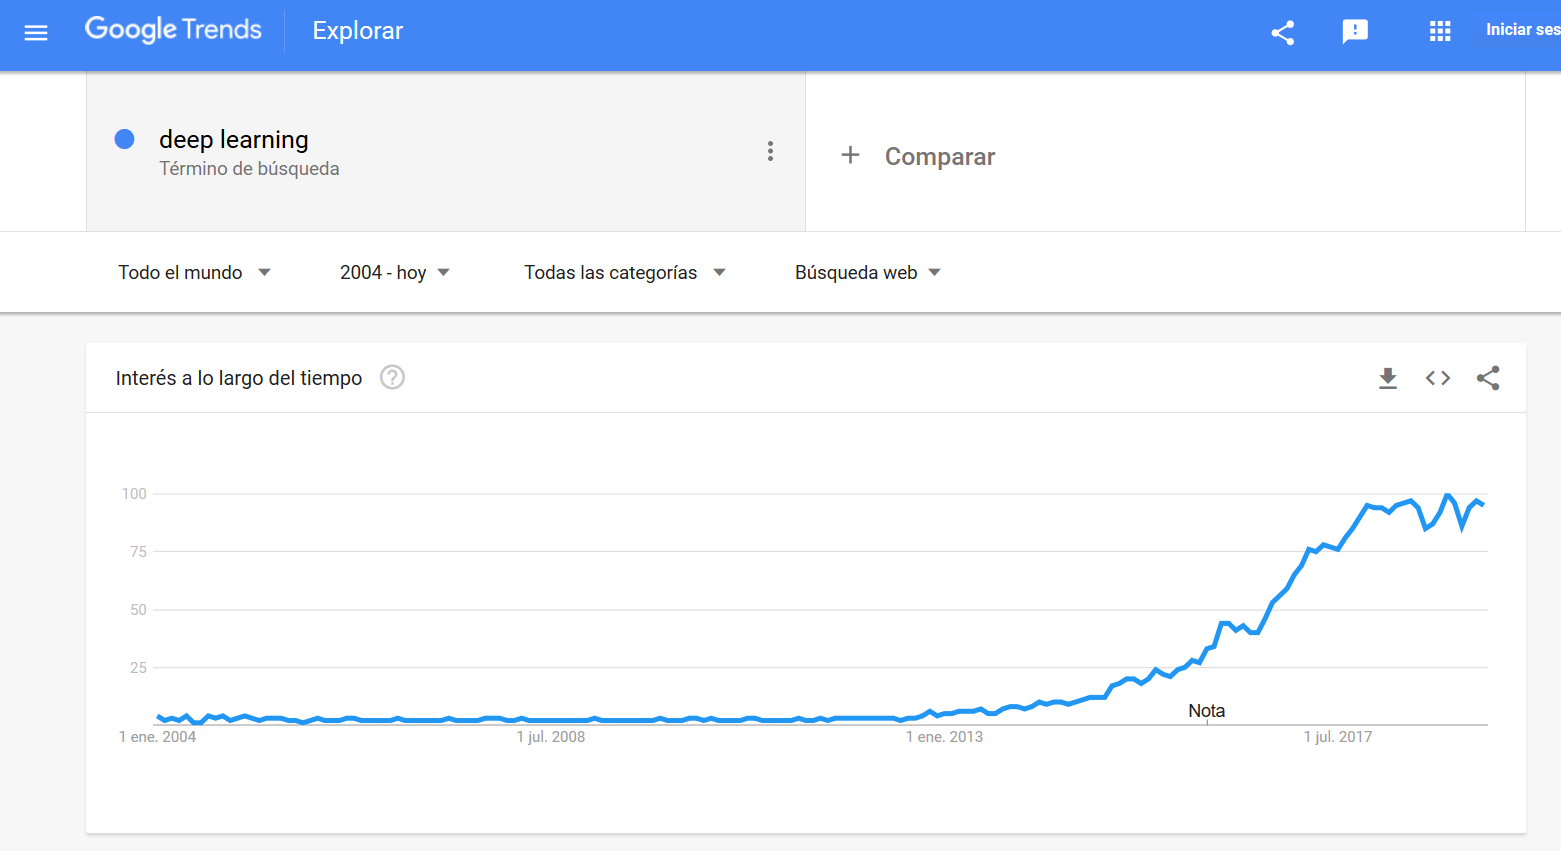
\includegraphics[width=1\textwidth]{growth.png}
    \caption{Búsquedas en google del termino \textit{Deep learning}}
    \label{fig:growth}
\end{figure}

En los últimos años, la capacidad de clasificar de algoritmos de \textit{deep learning} supera a la del ser humano\cite{DBLP:journals/corr/YangH15}, como muestra la figura \ref{fig:errorLSVRC}. En esta figura se muestra el error en el concurso del ganador de cada año, y también se muestra el error humano cometido. Se puede observar también como ha ido mejorando la tecnología muy rápidamente.


\begin{figure}[h]
    \centering
    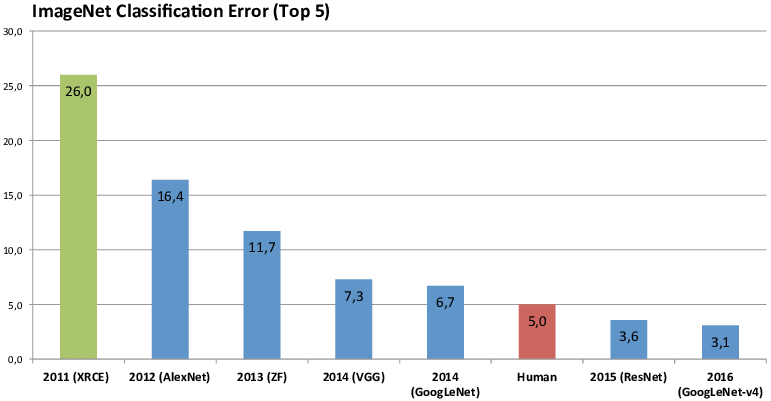
\includegraphics[width=1\textwidth]{Winner-results-of-the-ImageNet-large-scale-visual-recognition-challenge-LSVRC-of-the.png}
    \caption{Error de los ganadores del LSVRC los años 2011-2016}
    \label{fig:errorLSVRC}
\end{figure}

Estos resultados prometedores y su utilización en la resolución de problemas de vanguardia, como los coches autónomos, identificaciones faciales, por voz, etc,  ha hecho que no haya signos de ralentización en el campo y que hoy en día siga siendo interesante para investigar y trabajar, tanto en el ámbito público universitario como en el mercado privado, para aplicaciones más comerciales.


\subsection{Conclusiones}

Este campo ha sido uno de los más importantes del siglo pasado, pero ha tenido problemas en la investigación y varios parones, entre otras cosas por la falta de potencia de cada época. Además, al ser un campo multidisciplinar hizo que se publicara sobre él de forma desperdigada en muchas revistas, lo cual hacía el seguimiento por parte de la comunidad científica difícil. No solo eso, sino que ha cambiado de nombres múltiples veces. Básicamente, es lo mismo hablar de \textit{cybernetics} (proto-término acuñado en los 40 para referirse a este campo), redes neuronales artificiales (primera ola), redes neuronales (primera ola), \textit{conectionism} (segunda ola), y el más moderno, \textit{deep learning} (tercera ola).

\section{Acelerómetros}

Un acelerómetro es un dispositivo que mide la aceleración propia de un cuerpo. Esto quiere decir que en reposo, miden la aceleración de la fuerza de la gravedad en el eje de la tierra, normalmente z.

Su invención fue en 1784, por George Atwood. Se lo conocía como máquina de Atwood (ver figura \ref{fig:atwood}), y durante mucho tiempo, su utilidad era reducida a estudios científicos. Posteriormente, la industria del automóvil, en búsqueda de mayor eficiencia empieza a usarlos en sus vehículos para mejorarla.

\begin{figure}[h]
    \centering
    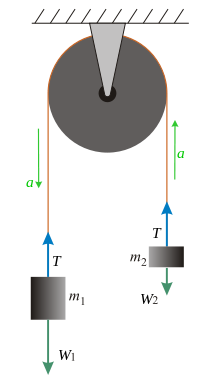
\includegraphics[scale=0.5]{atwood.png}
    \caption{Máquina de Atwood}
    \label{fig:atwood}
\end{figure}

El funcionamiento es sencillo, basado en la segunda ley de Newton.

\begin{equation}
m_1 g -T = m_1 a
\end{equation}
\begin{equation}
T - m_2 g = m_2 a
\end{equation}

De esta forma, si se suman ambas ecuaciones:

\begin{equation}
(m_1 -m_2)g = (m_1+m_2)a
\end{equation}

Y de ahí, si conocemos ambas masas, podemos obtener la aceleración.

Las necesidades de las industrias emergentes en el siglo XX, como la automovilística o la minería hicieron que hubiera un gran desarrollo a lo largo del siglo pasado.

\subsection{Primera era: 1923-1936}

El primer gran avance en el campo fue en 1923 cuando McCollun y Peters\cite{6534032} desarrollaron el primer acelerómetro moderno mediante un sistema de resistencias variables. Consistía en un sistema en forma de E que contenía entre 20 y 55 discos de carbono con un circuito de puente de Wheatstone que conectaba los dos extremos. En la figura \ref{fig:wheatstone} se puede observar un diagrama de este acelerómetro.

\begin{figure}[h]
    \centering
    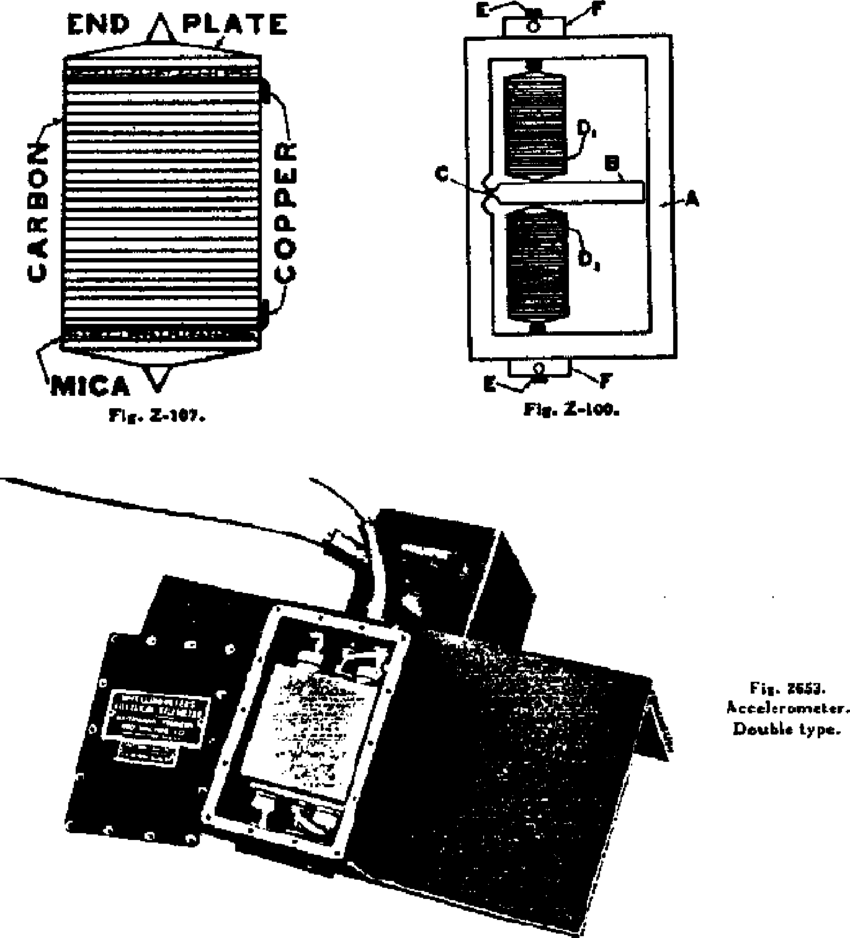
\includegraphics[scale=0.2]{mcculling.png}
    \caption{Diagrama del acelerómetro inventado por McCollun y Peters}
    \label{fig:wheatstone}
\end{figure}

Este dispositivo funciona con un efecto piezorresistivo. Este efecto provoca que el material cambie de resistencia eléctrica al ser sometido a una fuerza mecánica. El circuito puente de Wheatstone sirve para medir resistencias desconocidas entre los dos extremos, y sabiendo el cambio de la resistencia se obtiene la aceleración.

Durante los próximos años, el desarrollo de esta tecnología hace que se extienda moderadamente, sobretodo en la industria militar, la aviación y las empresas automovilísticas, pero estos dispositivos eran caros, lo que limitó su expansión.

\subsection{Segunda era: 1936-1950}
En 1936\cite{50yearsof} se inventó el acelerómetro basado en un extensómetro. Un extensómetro es un sensor que mide la deformación usando el efecto piezoresistivo que posee el material del que está construido.  Este tipo de dispositivos eran mucho más baratos y sencillos de hacer, lo que provocó que se extendieran por todas las industrias que los necesitaban pero no podían justificar los precios anteriores. De hecho, varias empresas de aviación se hacían sus propios dispositivos de manera interna.

El mayor problema que presentaban este tipo de acelerómetros es que ofrecían un rango de voltaje de 30 mV, por lo que dependiendo de la aplicación, la relación señal a ruido era muy mala. Para mejorar esto, se hacían los extensómetros muy finos, para tener la mayor flexibilidad posible, lo que hacía surgir otro problema, la fragilidad del sistema. Para solucionar esto, se dio una vuelta de tuerca, añadiendo un fluido amortiguante en el sistema, que limitara los rangos de vibración. De esta forma, se mejoraba la respuesta en frecuencia en un factor 3 y se reducía la amplificación de la frecuencia resonante a la mitad. Este método tenía contras, la mayor de ellas es debido a la introducción del liquido amortiguador, que provocó que la respuesta en frecuencia se hiciera muy dependiente de la temperatura, reduciendo la usabilidad de estos dispositivos a $\pm 20$ °C de la temperatura ambiente.

Todos estos problemas, la fragilidad del sistema, el bajo valor absoluto de las corrientes y el pequeño rango de temperaturas de funcionamiento incitaron a que se buscaran alternativas a esta tecnología. Además, tenían problemas para detectar las aceleraciones transitorias. Esto fue estudiado por Levi \textit{et al.}\cite{levy} en 1950 en un estudio encargado por la oficina nacional de estándares(ahora conocido como NIST, instituto nacional de estándares y tecnología) y financiado por la Marina estadounidense. 

\subsection{Tercera era: 1950-1991}

Estas limitaciones hicieron que se investigaran más a fondo otras tecnologías, entre ellas el efecto piezoeléctrico. El efecto piezoeléctrico es similar, en parte, al piezoresistivo, al recibir una fuerza mecánica, el dispositivo reacciona, pero  en este caso, tiende a separar las cargas entre las caras, creando una diferencia de potencial. Como vimos antes, los piezoresistivos cambiaban  su resistencia, y los piezoeléctricos generan un voltaje. Una gran ventaja que tienen es que los voltajes generados tienen un valor absoluto alto, por lo que trabajar con ellos es mucho más sencillo y el ruido pasa a ser un problema menor. Además, las frecuencias resonantes son muy altas, por lo que no hace falta amortiguarlas.

Estos dispositivos piezoeléctricos son los padres de nuestros sensores. Los materiales más típicos para su construcción son metales ferroeléctricos y cuarzo. Debido a la bajada de coste del sistema, empezó a surgir un mercado competitivo en el que varias empresas estaban innovando constantemente.

\subsection{Cuarta era: 1991-?}

Con la llegada de la era digital y mejores técnicas de fabricación, la tecnología de los acelerómetros evolucionó una vez más gracias a los sensores MEMS. Estas siglas se refieren a \textit{microelectromechanical system}, o sistema microlectromecánico. Esto no es más que la miniaturización de los sistemas electrónicos.. El primer acelerómetro MEMS como lo conocemos hoy en dia, salió al mercado en 1991, el ADXL 150. Los sensores MEMS tienen grandes ventajas frente al resto. Su tamaño es de escala micrométrica, por lo que son baratos de construir en masa y no ocupan mucho espacio. Son eficientes energéticamente hablando, ya que apenas consumen electricidad. Los acelerómetros MEMS utilizan materiales piezoeléctricos para realizar la misma medida que se haría con un sensor más grande de los anteriores, pero a escala microscópica. Para hacerse una idea, en la figura \ref{fig:acelerometro}, se muestra una imagen de un acelerómetro MEMS, el ADXL 362, que mide 3x3.25x1.06 mm.

\begin{figure}[h]
    \centering
    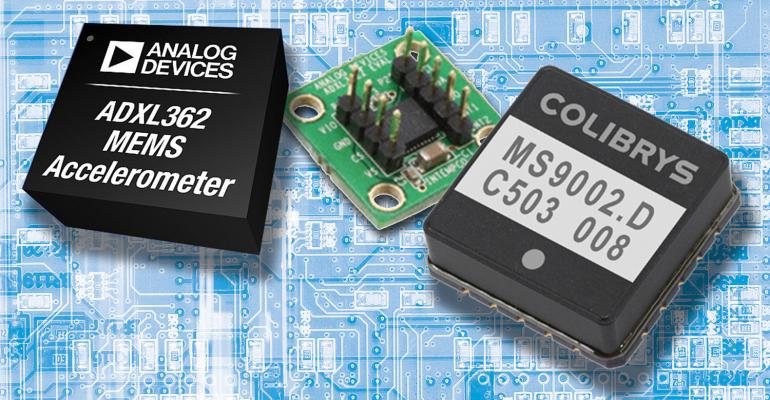
\includegraphics[width=1\textwidth]{MEMSpromo.jpg}
    \caption{Imagen de un acelerómetro MEMS}
    \label{fig:acelerometro}
\end{figure}

\subsection{Conclusiones}

Desde inicio del siglo anterior, la tecnología alrededor de los acelerómetros ha estado en constante avance, y sigue estando hoy en día. El desarrollo de los \textit{smartphones}, videojuegos y nuevas tecnologías, que requieren acelerómetros cada vez más precisos no ha hecho sino ayudar a una tecnología que ya estaba presente en el campo militar, médico, de investigación, automovilístico, etc. 

Actualmente, los acelerómetros, y todo este conjunto de sensores, como giroscopios, magnetómetros, barómetros etc, han cambiado nuestra forma de percibir el mundo. Estos dispositivos han permitido mecanizar muchas tareas, como el control de pacientes crónicos, automatización de regadíos, en aplicaciones más modernas como la conducción autónoma, realidad virtual... Es una tecnología con muchos frentes de investigación y con más cada día que pasa.

\section{Identificación de patrones movimiento}
Independientemente del tipo de movimiento que se quiera estudiar, normalmente el proceso para la identificación de un patrón se divide en tres partes: Tomar medidas con los sensores, extraer la información relevante de esos datos y finalmente procesarla y clasificarla. Las dos últimas se hacen a nivel de software. A continuación se describirá con más detalle este proceso, desde la captura de información hasta el resultado final clasificado.

\subsection{Captura de información: Sensores}
Se van a enumerar los sensores de los que dispone un \textit{smartphone} o un \textit{smartwatch} cualquiera.

\paragraph{Sensores de movimientos MEMS}

Al inicio, los \textit{smartphones} tenían solo un sensor de movimiento MEMS, un acelerómetro. Este sensor mide la aceleración debida a la gravedad y al movimiento del cuerpo a través de tres ejes ortogonales. Con este sensor se han podido implementar algoritmos para ver el número de pasos. En los siguientes años se fue imponiendo sensor mas complejo, llamado IMU, \textit{inertial measurement unit}. Esta tiene 6 grados de libertad, 3 ejes de acelerómetro y otros 3 de giroscopio. El giroscopio se encarga de medir la velocidad angular de los tres ejes, y permite detectar el cambio de orientación del dispositivo. Y ya, en estos últimos años, esta IMU ha sido ampliada a MIMU, en la que se le ha añadido un magnetómetro, añadiendo 3 grados de libertad extra.

\paragraph{Sensores ambientales MEMS}

Anteriormente se mencionó el magnetómetro, pero aunque está en el sensor de movimiento, es un sensor ambiental, ya que su medida depende de la posición del usuario con respecto al campo magnético terrestre. Así permite orientar el \textit{wearable} con respecto al campo magnético de la tierra, y por tanto saber su posición exacta en reposo.

Además del magnetómetro, está el barómetro, que puede usar para determinar la diferencia de altura del usuario entre distintos momentos, o la presión ambiental, y saber la altura con respecto al mar a la que se encuentra.

Las ventajas de estos sensores es que no son invasivos y gasta poca batería su uso continuado, esto hace que sean ideales para hacer el sistema.

\paragraph{Otros sensores} Otros sensores que poseen este tipo de dispositivos son los audiovisuales, cámara y micrófono, el sensor de posicionamiento GPS (ha mejorado notablemente en los últimos años \cite{vonWatzdorf:2010:APD:1899662.1899664}) y el sensor PPG (\textit{photoplethysmography}), que sirve para medir las pulsaciones con sorprendente precisión\cite{7748986}\cite{77489867}. Estos sensores no van a ser usados en este trabajo, pero existen y pueden ser usados para la detección del ambiente que rodea al usuario\cite{Lu:2009:SSS:1555816.1555834} o simplemente tener una imagen más completa del movimiento del usuario\cite{doi:10.1155/2014/503291}.

\subsection{Desarrollo del algoritmo}
Inicialmente los modelos que se desarrollaban para ver el estado de movimiento eran clasificadores heurísticos, por ensayo y error. Esto se debía a que los \textit{smartphones} iniciales tenían una capacidad de procesamiento limitada. Sin embargo, los \textit{smartphones} modernos tienen la potencia como para ejecutar algoritmos modernos de extracción de datos y modelos de clasificación.

Estos modelos son entrenados con diversos MLAs (\textit{Machine learning algorithms}). Estos algoritmos analizan los datos de entrada durante un proceso supervisado de aprendizaje que defina la función o reglas que se usan para clasificar el movimiento, en este caso los distintos tipos que hay. Algunos de los MLAs usados son:

\begin{itemize}
\item Modelo oculto de Markov
\item K vecinos más próximos
\item Maquinas de vectores de soporte
\item Redes Bayesianas
\item Modelos gausianos de combinación
\item Regresiones logísticas
\item Clasificador bayesiano ingenuo
\item Árbol de decisiones
\item Redes neuronales.
\end{itemize}

\paragraph{Modelo oculto de Markov} Este modelo asume que el sistema a estudiar es un proceso de Markov con parámetros desconocidos. Un proceso de Markov es un fenómeno aleatorio dependiente del tiempo para el cual se cumple la propiedad de Markov, que es que la variable a estudiar no tiene memoria. Esto implica que la probabilidad condicional sobre el estado presente, pasado y futuro son independientes.

\paragraph{K vecinos más próximos} Es un modelo de reconocimiento de patrones. El caso de los más próximos es no parámetrico, ya que clasifica en función de la cercanía. Si es clasificador, la salida del modelo es la clase a la que pertenece. Si es de regresión, la salida es el valor de una propiedad del objeto estudiado. Ese valor es la media de los k vecinos más cercanos.

\paragraph{Maquinas de vectores de soporte} Estos algoritmos son modelos de aprendizaje supervisado que analizan los datos y separan los datos en distintos sectores. A partir de ese entrenamiento, posteriormente se van separando los datos de entrada entre las distintas secciones.

\paragraph{Redes Bayesianas} Son modelos probabilísticos de grafos, que representan unas variables, sus dependencias condicionales mediante un grafo directo. Un ejemplo seria las enfermedades y sus síntomas. Unos síntomas dados obtendrían la enfermedad que está afectando al individuo.

\paragraph{Regresiones logísticas} Usa una función logística para obtener un modelo de varias variables.

\paragraph{Clasificador bayesiano ingenuo} Es parecido al modelo de redes bayesianas, pero se simplifica haciendo que haya mas independencia entre las distintas clases de objetos a estudiar.

\paragraph{Árbol de decisiones} Usa un árbol como modelo predictivo para obtener a partir de observaciones de un objeto conclusiones.

\paragraph{Redes neuronales} Son un algoritmo basado en las neuronas. Aprenden independientemente a partir de un conjunto de datos de entrada a distinguir que es lo que los une o separa.

De entre todos estos, aquí se van a usar las redes neuronales, por eso se va a hacer una sección ampliando la información sobre éstas posteriormente. Se va a usar las redes neuronales porque se ha probado que son eficaces para este tipo de problemas\cite{s131013099} con exactitudes de hasta el 87\%. Esto es así porque las redes neuronales son una herramienta muy potente para la clasificación o separación de distintos eventos. Son potentes aprendiendo patrones de comportamiento, y no los comportamientos en si, que es lo interesante aquí, ya que no todas las personas van a andar igual, o saltar o caerse de la misma forma, sin embargo los patrones si van a ser similares.

\subsection{Limitaciones}

Son muchos sensores de los que dispone un sistema Android, usarlos todos en todo momento nos daría una imagen perfecta o casi perfecta de la situación de movimiento del usuario. Sin embargo usarlos todos constantemente conlleva problemas. Nos centraremos aquí en el consumo de batería y en las limitaciones de los modelos.

\paragraph{Consumo de batería}
Durante los últimos años se ha visto aumentada la potencia de los \textit{smartphones} constantemente, pero hay un aspecto que ha empeorado, el tiempo de uso antes de que se agote la batería. Compárese un dispositivo mas antiguo, previo a los \textit{smartphones}, como puede ser cualquier Nokia clásico y cualquier teléfono actual. En duración de batería gana sobradamente el Nokia. 

Ésto implica que poner a trabajar todos los sensores y el procesador con los datos es fatal para la duración de batería del dispositivo. Debido a ello se utilizan alternativas al recoger todo y analizar. 

Hablando de esto, se ha estudiado que hay tres factores que afectan al gasto de batería de un \textit{smartphone}, el primero es el número de interacciones entre el usuario y el \textit{smartphone}, el segundo las aplicaciones instaladas y usadas por el usuario y finalmente el hardware y el sistema operativo del terminal\cite{Falaki:2010:DSU:1814433.1814453}. Además, se ha estudiado que en estado de suspensión, pantalla apagada pero \textit{smartphone} encendido, el principal consumidor es el módulo encargado de la conexión por datos a internet. Por el contrario, si el teléfono está encendido, pero en \textit{idle}, es decir, no tiene aplicaciones en segundo plano, es el procesador gráfico lo que más consume\cite{Carroll:2010:APC:1855840.1855861}. Se puede observar en la figura \ref{fig:consumo} gráficamente.
\begin{figure}[h]
    \centering
    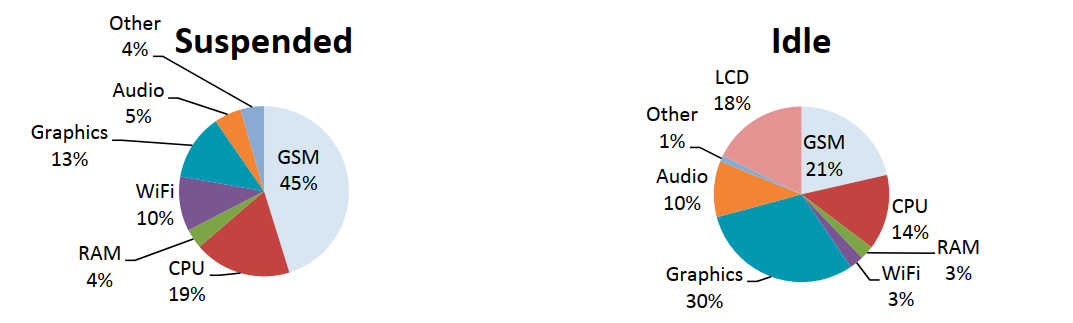
\includegraphics[width=1\textwidth]{batterylife.png}
    \caption{Consumo de batería de un \textit{smartphone}\cite{Carroll:2010:APC:1855840.1855861}}
    \label{fig:consumo}
\end{figure}

\paragraph{Modelos de posición fija}
Una limitación a la hora de modelar el movimiento de un usuario usando un \textit{smartphone} es que su posición no es fija, puede estar en distintas partes del cuerpo, como se ve en la figura \ref{fig:posiciones} y nuestro algoritmo debe tenerlas en cuenta. Tienen ventajas e inconvenientes. 

\begin{figure}[h]
    \centering
    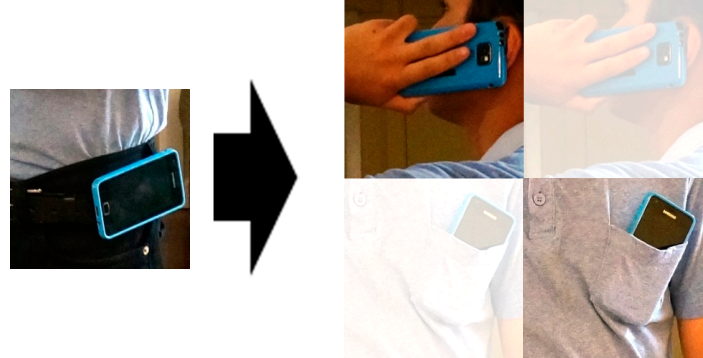
\includegraphics[width=1\textwidth]{position.png}
    \caption{Ejemplo de distintas posiciones de un \textit{smartphone}.}
    \label{fig:posiciones}
\end{figure}



Si se usa un algoritmo de posición fija, se obliga al usuario a tener que llevar el dispositivo de una determinada forma siempre, fijo, pero a cambio, al saber su posición exacta el algoritmo puede ser mucho mas preciso, ya que toma en cuenta principios de la biomecánica aplicados a esa zona concreta. Aunque si el objetivo es el estado de movimiento, el \textit{smartphone} ha de estar lo más cerca posible del centro de masas, por eso la mayoría de los estudios tienen el \textit{smartphone} fijo en un cinturón\cite{5673816}.

Se han hecho estudios aplicados a deportes y similares en los que al estar el dispositivo en una posición fija, se puede detectar perfectamente el tipo de movimiento. Hay aplicaciones para el fútbol\cite{s130405317} y el hockey, la natación\cite{Marshall:2013:SSD:2494091.2496036}, y como entrenador personal en un gimnasio colocando el \textit{smartphone} una tabla de equilibrios\cite{KRANZ2013203}.

\paragraph{Modelos de posición dependiente}

Estos modelos son una pequeña variación del anterior, en el cual se supone que el dispositivo va a estar alrededor de unas zonas concretas. Permiten que el dispositivo no esté absolutamente fijo, lo cual es una comodidad para el usuario. Además no pierden mucha exactitud. Estos modelos ya apenas se usan, fueron un avance del anterior en comodidad para el usuario, pero al final, son un parche sobre el problema, que lo alivia pero no lo soluciona. Los usuarios solo pueden tener el dispositivo en ciertas posiciones, no todas.

\paragraph{Modelos independientes de la posición}

En estos modelos, no importa la posición del dispositivo con respecto al usuario. Son los más cómodos para éste pero pierden capacidad. Por ejemplo, hay estudios en los que se detectan bien hasta siete tipos de movimiento, pero luego los estacionarios típicos como de pie, sentado y tumbado no es capaz de hacerlo\cite{6488584}.% 

\subsection{Conclusiones}

Como se ha podido ver, hay muchos algoritmos de inteligencia artificial, y muchos sensores dentro de un smartphone, pero las limitaciones en el consumo de batería hace que no se puedan usar todos.

En nuestro caso, el algoritmo a utilizar es un modelo de posición fija, ya que es el evidente a usar en un \textit{smartwatch}. El sensor que se va a utilizar es el acelerómetro, porque es el que mejor se ajusta a las necesidades del proyecto, por los datos que ofrece y por el poco gasto de batería que produce. Y el sistema de aprendizaje se usará una red neuronal, ya que ha demostrado en estudios anteriores que es un algoritmo que ha sido probado ya en estudios anteriores.


\chapter{Fundamentos teóricos}
\section{Introducción a las redes neuronales}
\subsection{Definición}
Las redes neuronales son una herramienta matemática basada vagamente en una neurona. Son redes de elementos que utilizan algoritmos de aprendizajes.

\subsection{Estructura biológica}

\begin{figure}[h]
    \centering
    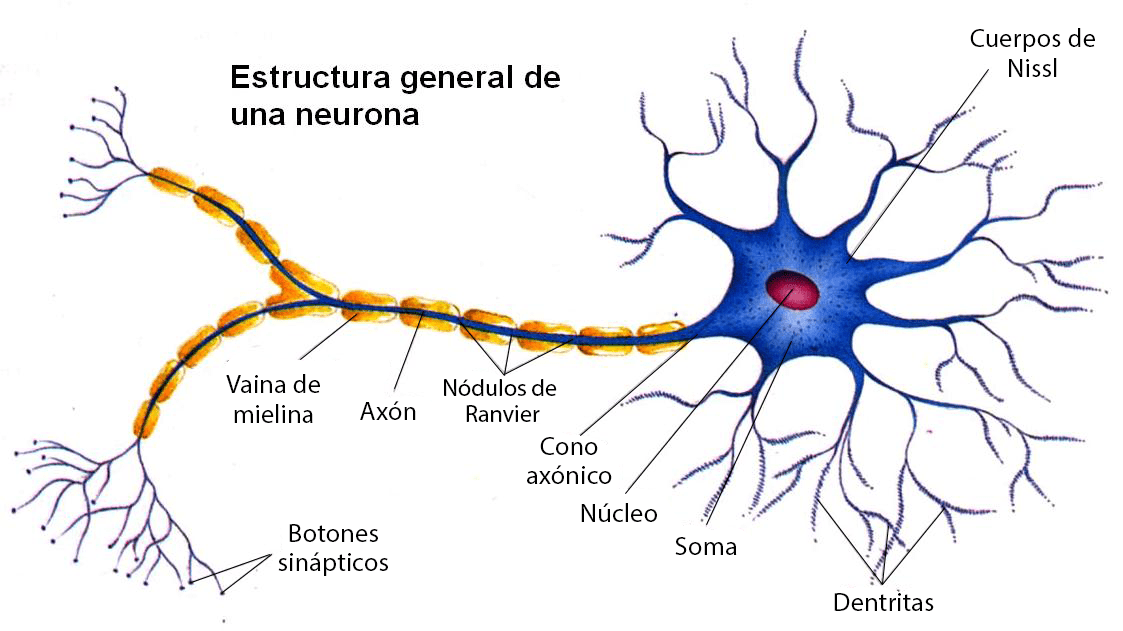
\includegraphics[width=1\textwidth]{estructura_general_neurona.png}
    \caption{Estructura del una neurona.}
    \label{fig:neuronareal}
\end{figure}

Se puede observar en la figura \ref{fig:neuronareal} que una neurona es muy distinta a la célula típica. Lo más importante de una neurona es que está unida a otras muchas mediante las dendritas y los botones sinápticos. La neurona se excita por las dendritas mediante un proceso llamado sinapsis, que consiste en el intercambio de neurotransmisores en ellas. Esto provoca un impulso nervioso, que se transmite posteriormente por el axón hasta los botones sinápticos, que están conectados a otras neuronas o músculos.

El axón es el elemento alargado, rodeado por vainas de mielina y éstas acaban en los nódulos de Ranvier. Las vainas de mielina son células de Schwann y actúan de encapsuladores de la señal, haciendo que la señal no se pierda. Los nódulos de Ranvier son los huecos que quedan en el axón entre células de Schwann. Estos 'huecos' están llenos de iones que amplifican la señal.

\begin{figure}[h]
    \centering
    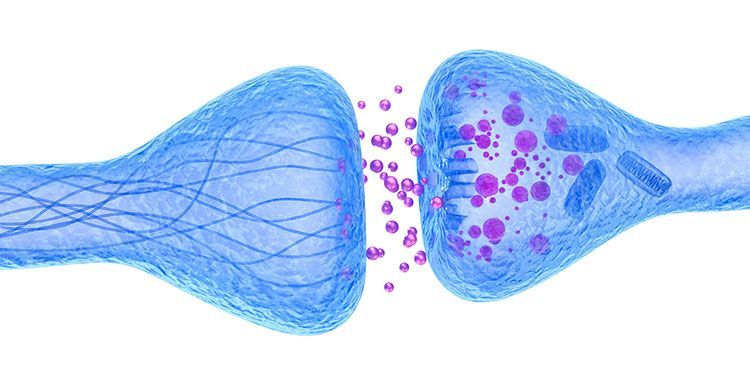
\includegraphics[width=0.8\textwidth]{sinapsis.jpg}
    \caption{Sinapsis de una neurona.}
    \label{fig:mesh2}
\end{figure}

Además, las neuronas tienen un comportamiento más a tener en cuenta. No están constantemente trabajando, sino que tienen fases de descansos. A estas fases se le llaman estado refractario. Es el tiempo necesario tras una estimulación necesario para recuperar el estado inicial previo y en el cual no puede volver a ser excitada. Se puede ver en la figura \ref{fig:refractario} las fases de activación de una neurona.
\begin{figure}[h]
    \centering
    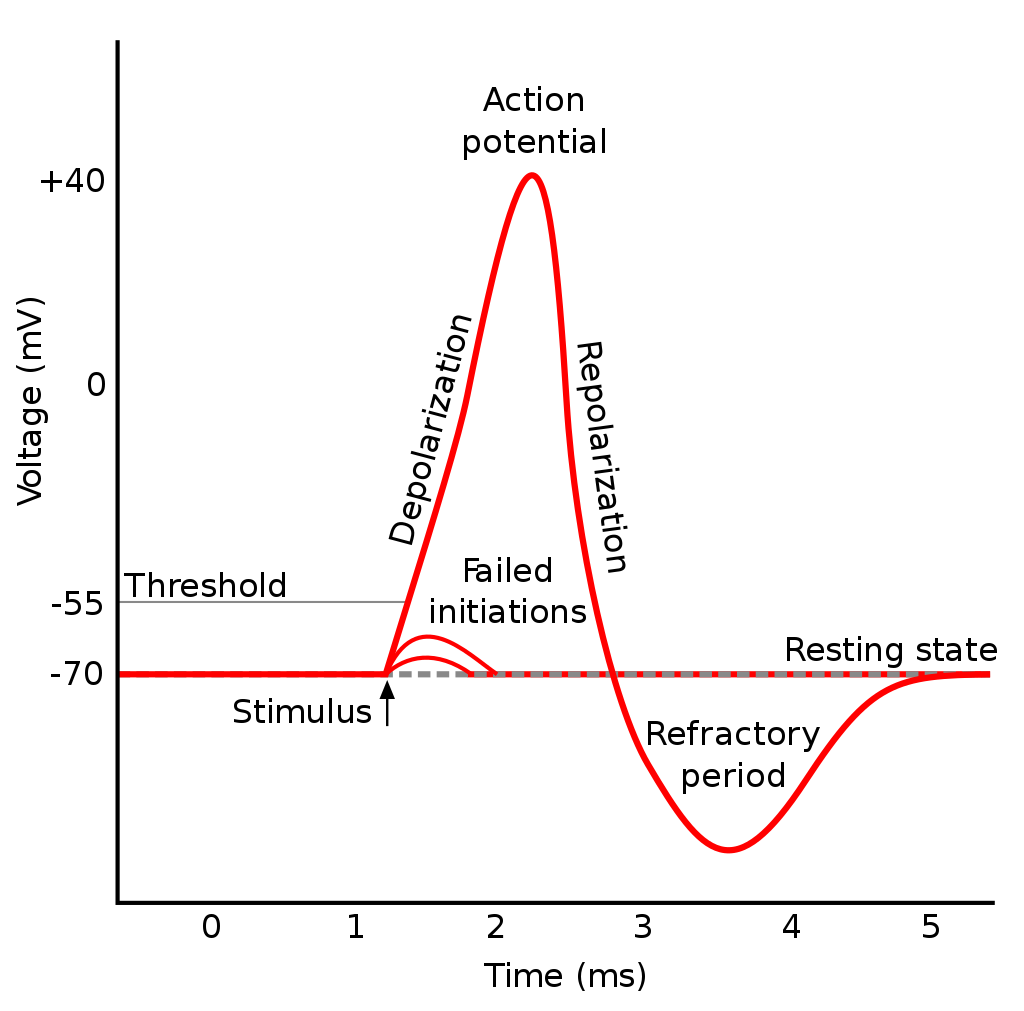
\includegraphics[scale=0.2]{refractorystate.png}
    \caption{Estado refractario.}
    \label{fig:refractario}
\end{figure}

Que en una neurona suele durar 1 milisegundo. Todo esto hace que las neuronas sean una célula de especial interés, ya que tiene una estructura interesante que puede ser reproducida matemáticamente, aunque evidentemente las neuronas reales son más complejas que las de los algoritmos.

La sinapsis es el proceso más importante, ya que el 'peso' de cada sinapsis, y a quien se tiene que transmitir esa señal es decidido en la neurona muy rápidamente. Además, la sinapsis tiene distintos orígenes, químicos o eléctricos. La neurona puede trabajar con neurotransmisores que son sustancias químicas como la dopamina, o puede ser eléctrica directamente, mediante la transmisión directa de iones.	

Además, la sinapsis puede tener tres clases, excitadora, que incrementa la energía, 	inhibidora, que la reduce y moduladora, que es la que cambia el patrón o la frecuencia de la actividad de la que se ocupe ese grupo de neuronas. 

\subsection{Estructura en el software}

El interés en las redes neuronales lleva tanto como la computación moderna. Los algoritmos son antiguos pero siempre ha existido la limitación en el hardware, ya que consisten en muchos procesos ejecutándose en paralelo. Los primeros algoritmos son de los 50-60. El más importante de ellos es el de Perceptrón. El Perceptrón es un algoritmo de aprendizaje supervisado de un clasificador binario. Esto es, un algoritmo que dependiendo de la entrada, puede decidir la clase de elemento que es. Fue inventado por Rosenblatt como una estructura monocapa con una función de activación estilo escalón.

La función de activación es la que define el comportamiento de una neurona. De la función de activación depende el funcionamiento de la neurona y sobretodo los resultados que da. En una función escalón el resultado va a ser Si o No, 0 o 1. Sin embargo, la función puede ser Gaussiana, la identidad, una tangente... Depende del problema a resolver y del algoritmo.

A partir del algoritmo del perceptrón se desarrolla en los 80 el perceptrón multicapa. Este es el algoritmo más importante del campo, y tiene ya 40 años. Este algoritmo tiene una capa de entrada, una de salida y las que sean necesarias entre media.

\begin{figure}[h]
    \centering
    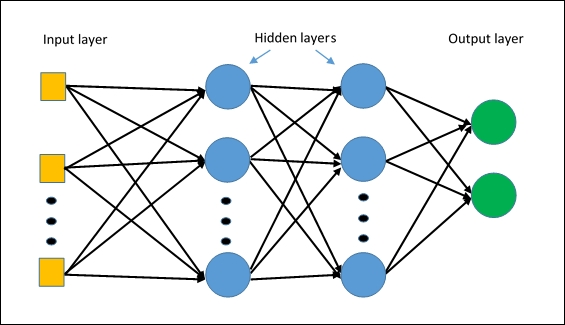
\includegraphics[width=0.7\textwidth]{multicapa.jpg}
    \caption{Estructura de un perceptrón multicapa.}
    \label{fig:estructuraneurona}
\end{figure}

La estructura del algoritmo es similar a la de la figura \ref{fig:estructuraneurona}, donde lo más importante es que cada neurona está conectada a todas las neuronas de la capa anterior y posterior. Lo interesante de este algoritmo es que cada capa puede tener una función de activación distinta y ocuparse de una función distinta. Al ser muy genérico, el perceptrón multicapa puede ser usado en muchos problemas simplemente adaptando el número de capas internas o la función que cumplen. Hasta hace poco, hacer un modelo con mucha profundidad de capas era muy caro a nivel de hardware, pero con el aumento de potencia y de la potencia en la nube, ha hecho que resurja el campo de investigación, mas centrado en la resolución de problemas complejos y muchas capas para ello, conocido como \textit{deep learning}. La limitación de hardware ha sido ahora sustituida por una computación en la nube muy barata que se puede alquilar a Amazon Cloud o Google y ha revolucionado el campo.

\begin{figure}[h]
    \centering
    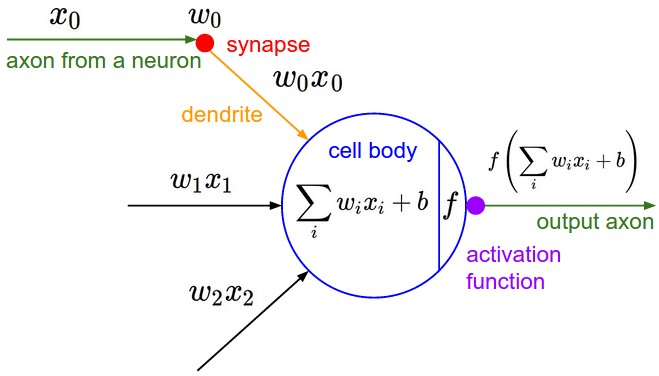
\includegraphics[width=0.7\textwidth]{neuron.jpg}
    \caption{Estructura de una neurona.}
    \label{fig:estructura}
\end{figure}

El funcionamiento básico de cada elemento en una red es similar al de la figura \ref{fig:estructura}, cada 'neurona' le llegan los axones de otras neuronas(la capa anterior a ella) con unos valores $x_0$ sobre los que se aplica un peso $w_0$, de forma que se normaliza, y luego se ve si activa la función de activación y se transmite a las neuronas de las siguientes capas por su 'axón'. El valor $b$ es un umbral, que sirve para cambiar el punto de activación.

La capacidad de aprender de la neurona consiste en preparar los pesos $w_i$ en un proceso de entrenamiento. En los pesos sinápticos es donde está la profundidad del tema. Hay dos formas de entrenar una neurona, mediante un aprendizaje supervisado o mediante un aprendizaje no supervisado. El caso del aprendizaje supervisado, se entrega a una red neuronal los datos de entrada y de salida y mediante el proceso de aprendizaje adapta los pesos para obtener los resultados. En el caso de un aprendizaje no supervisado, se le dan los datos y la red lo clasifica ella sola. Lo importante en el caso del aprendizaje supervisado es entregar unos buenos datos clasificados, y en el caso de un aprendizaje no supervisado, lo importante es el análisis posterior, ver en que se ha basado la red para clasificarlos, que a veces es de formas que no se esperan.

\subsection{Algoritmo de entrenamiento: Backpropagation}
Para entrenar la red se utiliza un algoritmo conocido como \textit{backpropagation}, o en español retropropagación. Esto es así porque se entrena primero a la capa más profunda(la más cercana a la salida) y posteriormente se van ajustando los errores de la anterior.

El aprendizaje consiste en introducir los datos de entrada, comparar con los de salida y ver el error cometido. Posteriormente se intenta minimizar ese error. El aprendizaje pues es ajustar los pesos sinápticos para minimizar el error. El aprendizaje puede hacerse de dos formas, por lotes se hace un error global al presentar todos los patrones, e incremental, en el que se presentan los patrones uno a uno y se adaptan los pesos a cada patrón. Nuestros datos son:

\begin{equation}
x^P = [x_i^P] \; i= 1,..., N_e
\end{equation}
\begin{equation}
d^P = [d_k^P] \; k=1,...,N_s
\end{equation}

Donde las X son un conjunto de datos de entrada, y las D la salida para el conjunto de datos de entrada anterior. $N_s$ representa el número de salidas y $N_e$ el número de entradas. Ademas, al valor b, umbral, se le considera un peso más, $w_0$. Para empezar, se le entrega a la red el patrón de entrada $x^P$, y se obtiene una salida:

\begin{equation}
y_k^P=\Psi _s(z^P_k)=\Psi _s
\end{equation}

Donde $\Psi$ es la función de activación de la ultima capa. Ahora se compara cada dato con el valor de salida real, y se obtiene un error:

\begin{equation}
e^P_k=d_k^P-y_k^P
\end{equation}

El error global obtenido tiene en cuenta el de todas las neuronas, y se representa de forma cuadrática:

\begin{equation}
E^P = \frac{1}{2} \sum_{k=1}^{N_s} (e_k^P)^2=\frac{1}{2}\sum_{k=1}^{N_s}(d_k^P-y_k^P)^2
\end{equation}

Y finalmente se modifican los pesos sinápticos para minimizar el error:

\begin{equation}
w_{kj}(t+1)=w_{kj}(t) + \Delta w_{kj}(t+1)
\end{equation}

La forma de calcular $\Delta w_{kj}(t+1)$ es la que define al algoritmo de adaptación(aprendizaje). El algoritmo debe modificar todos los pesos de todas las neuronas de todas las capas de la red. Como solo se conoce el error en la salida, es necesario empezar por el final, a continuación se calculan los errores de la capa anterior, donde se considera el resultado obtenido en la capa de salida como el correcto y se ve el error con el calculado en la capa anterior. Así, sucesivamente, se llega hasta la primera capa. Esta forma de calcular es la que hace que se llame al método \textit{Backpropagation}. 

Primero hay que ver como varía el error en función de los pesos. Para ello hacemos el gradiente de la función de error respecto a los pesos

\begin{equation}
\nabla E^P = \frac{\partial E^P}{\partial w_{kj}}
\end{equation}

Aplicamos la regla de la cadena:

\begin{equation}
\frac{\partial E^P}{\partial w_{kj}} =  \frac{\partial E^P}{\partial e_{k}^P} \frac{\partial e^P_k}{\partial y_{k}^P} \frac{\partial y^P_k}{\partial z_{k}^P} \frac{\partial z^P_k}{\partial w_{kj}}
\end{equation}

El valor del primer termino es:

\begin{equation}
\frac{\partial E^P}{\partial e_{k}^P} =  \frac{\partial}{\partial e_k^P}\left(\frac{1}{2} \sum_{k=1}^{N_s} (e_k^P)^2\right) = e^P_k=(d_k^P-y_k^P)
\end{equation}

El segundo:

\begin{equation}
\frac{\partial e^P_k}{\partial y_{k}^P} = \frac{\partial}{\partial y_{k}^P}\left(d^P_k - y^P_k\right) = -1
\end{equation}

Tercero: 

\begin{equation}
\frac{\partial y^P_k}{\partial z_{k}^P} = \frac{\partial \Psi _s(z_k^P)}{\partial z_{k}^P} = \Psi _s'(z_k^P)
\end{equation}

Finalmente, el cuarto:

\begin{equation}
\frac{\partial z^P_k}{\partial w_{kj}}=\frac{\partial \left(\sum_{j=0}^{N_e} w_{kj} y_j^P\right)}{\partial w_{kj}} = y_j^P
\end{equation}

Recomponiendo se llega a:

\begin{equation}
\frac{\partial E^P}{\partial w_{kj}} =
-(d_k^P-y_k^P) \cdot \Psi _s'(z_k^P) \cdot y_j^P
\end{equation}

Ahora se define la sensibilidad de la neurona k-ésima ante el patrón de entrada P($\delta_k^P$) como:

\begin{equation}
\delta _k^P = - \frac{\partial E^P}{\partial e^P_k}=-
\frac{\partial E^P}{\partial e_{k}^P} \frac{\partial e^P_k}{\partial y_{k}^P} \frac{\partial y^P_k}{\partial z_{k}^P} = (d_k^P-y_k^P) \cdot \Psi _s'(z_k^P)
\end{equation}

De forma que finalmente, la expresión del gradiente de error queda como:

\begin{equation}
\frac{\partial E^P}{\partial w_{kj}} = \delta_k^P \cdot y_j^P
\end{equation}

Para que la variación del peso haga disminuir la función de error, el error ha de ser proporcional al gradiente negativo de la función de error respecto a los pesos:

\begin{equation}
\Delta w_{kj}(t+1) = -\eta \frac{\partial E^P}{\partial w_{kj}} = \eta \delta_k^P y_j^P
\end{equation}

Donde $\eta$ es una constante de proporcionalidad cuyo valor se ajusta para adaptar la velocidad y precisión del aprendizaje. Con esto tenemos el algoritmo de la capa de salida. Ahora para hacer la ultima capa oculta, que no tiene ninguna dificultad desde el punto conceptual, pero si matemática:

\begin{multline}
E^P = \frac{1}{2} \sum_{k=1}^{N_s} (e_k^P)^2=\frac{1}{2}\sum_{k=1}^{N_s}(d_k^P-y_k^P)^2 =  \frac{1}{2} \sum_{k=1}^{N_s} \left(d_k^P - \Psi _s(z_k^P)\right)^2 =\\
\quad = \frac{1}{2} \sum_{k=1}^{N_s} \left(d_k^P - \Psi _s \left[ \sum_{j=0}^{N_s} w_{kj} y_j^P\right]\right)^2 = \\
\qquad \qquad = \frac{1}{2} \sum_{k=1}^{N_s} \left(d_k^P - \Psi _s \left[ \sum_{j=0}^{N_s} w_{kj}\Psi _{s-1}(z_j^P)\right]\right)^2 =\\
= \frac{1}{2} \sum_{k=1}^{N_s} \left(d_k^P - \Psi _s \left[ \sum_{j=0}^{N_s} w_{kj}\Psi _{s-1} \left\langle \sum_{l=0}^{N_s'} w_{jl} y_l^P\right\rangle \right] \right)^2
\end{multline}

A partir de esta expresión, se puede obtener, para el cálculo del gradiente del error:

\begin{equation}
\frac{\partial E^P}{\partial w_{jl}} = \frac{\partial E^P}{\partial e_{k}^P} \frac{\partial e^P_k}{\partial y_{k}^P} \frac{\partial y^P_k}{\partial z_{k}^P} \frac{\partial z^P_k}{\partial y_j^P} \frac{\partial y^P_j}{\partial z_j^P} \frac{\partial z^P_j}{\partial w_{jl}}
\end{equation}

Y calculando las derivadas, como en el caso anterior, una a una, se llega a:

\begin{equation}
\frac{\partial E^P}{\partial w_{jl}} =-\sum _{k=1}^{N_s}(d_k^P-y_k^P) \cdot \Psi ' _s(z_k^P) \cdot w_{kj} \cdot \Psi '_{s-1}(z_j^P) \cdot y_l^P
\end{equation}

Definiendo de nuevo la sensibilidad:

\begin{equation}
\delta _j^P = -\sum _{k=1}^{N_s}(d_k^P-y_k^P) \cdot \Psi ' _s(z_k^P) \cdot w_{kj} \cdot \Psi '_{s-1}(z_j^P)
\end{equation}

Obtenemos, finalmente:

\begin{equation}
\frac{\partial E^P}{\partial w_{jl}} = \delta _j^P \cdot y_l^P
\end{equation}

Y el resultado de la variación de pesos sería: 

\begin{equation}
\Delta w_{jl} = -\eta \frac{\partial E^P}{\partial w_{jl}} = \eta \cdot \delta _j^P \cdot y_l^P
\end{equation}

De esta forma se va iterando de forma que cada neurona de cada capa tiene una sensibilidad distinta adaptada a ella.

\section{Acelerómetros}

En la sección de antecedentes, se mostró que los acelerómetros están basados en una máquina de Atwood, que es un mecanismo muy sencillo.

Un acelerómetro digital no es muy distinto, se puede ver un diagrama en la figura \ref{fig:piezoelectric}.

\begin{figure}[h]
    \centering
    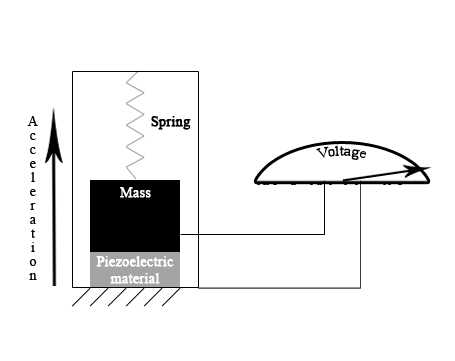
\includegraphics[scale=0.8]{piezoelectric.png}
    \caption{Acelerómetro piezoeléctrico.}
    \label{fig:piezoelectric}
\end{figure}

Los dispositivos piezoeléctricos tienen muchas aplicaciones debido a su generalidad. Son buenos sensores de presión, de aceleraciones, de otro tipos de fuerzas mecánicas. En la figura \ref{fig:piezotypes} se pueden observar algunos sistemas reales.

\begin{figure}[h]
    \centering
    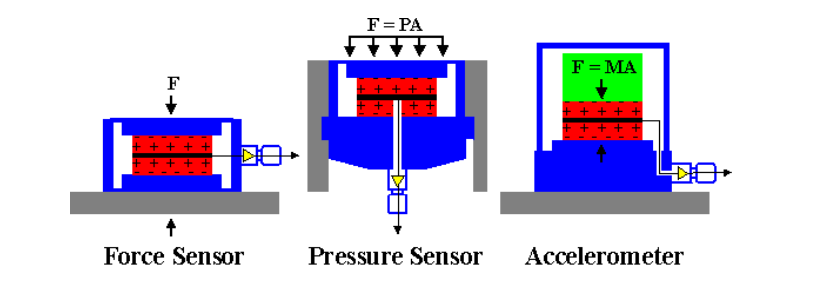
\includegraphics[width=1\textwidth]{piezoelectrictypes.png}
    \caption{Distintos tipos de dispositivos piezoeléctricos.}
    \label{fig:piezotypes}
\end{figure}


Tratando el tema con mayor rigurosidad, la naturaleza del efecto piezoeléctrico se debe en gran parte a la cantidad de dipolos que posee el material. Estos dipolos pueden ser inducidos por los iones que posee la red cristalina del material o debido a la presencia de grupos moleculares con propiedades eléctricas. Normalmente, un dipolo es un vector $\vec{P}$, por lo que tiene un valor y una dirección en función de las cargas que le rodean. Además, estos vectores suelen tomar el valor de sus vecinos, formando lo que se conoce como dominios magnéticos o de \textit{Waiss}. 

Estos dominios son aleatorios normalmente, de forma que el dipolo total se anula. Estos dominios pueden ser alineados aplicando un fuerte campo eléctrico DC al material, mediante el proceso de histéresis, por el cual los dipolos conservan la orientación que indujo el campo eléctrico en ausencia de él. Sin embargo, este proceso no es siempre posible, y algunos materiales no pueden ser alineados mediante este método. La razón por la que un material piezoeléctrico genera un voltaje es que cuando una fuerza mecánica es aplicada, la estructura cristalina es alterada, y cambia la dirección del vector $\vec{P}$. Dependiendo de la naturaleza de los dipolos, este cambio puede ser debido a la recolocación de los iones de la estructura cristalina o debido a la reorientación de los grupos moleculares con propiedades eléctricas.

Estos materiales pueden ser naturales o artificiales. El más común entre los naturales es el cuarzo, pero los artificiales son mas eficientes y normalmente cerámicos. Debido a su compleja estructura, su fabricación requiere precisión y seguir unos pasos muy concretos.

Es importante mencionar que los materiales piezoeléctricos solo presentan ese efecto si la temperatura es inferior a la temperatura de Curie. A mayor temperatura, el cristal presentaría una estructura cúbica simétrica simple, por lo que no habría mas momento dipolar.

\subsection{Fundamento matemático}

Un material piezoeléctrico genera un campo eléctrico interno cuando es sometido a una fuerza, y por el contrario, el material es sometido a una fuerza cuando se le aplica un campo eléctrico. Estas reacciones pueden darse en ambos sentidos. Lo que significa que dependiendo del material, un campo eléctrico en una dirección podría provocar una reacción mecánica en cualquier dirección. Esto implica, normalmente, ecuaciones tensoriales. Sin embargo, para simplificar los cálculos, se tomará el caso de un material, que solo puede producir un campo eléctrico en una dirección, con sentido paralelo o perpendicular en función del tipo de fuerza que es aplicada. Las ecuaciones son pues, considerando poca variación en temperatura y frecuencias bajas:
\begin{equation}
\vec{D} = d_1 \vec{T} + \epsilon ^T \vec{E}
\end{equation}
\begin{equation}
\vec{S} = s^E \vec{T} + d_2 \vec{E}
\end{equation}

Donde $\vec{D}$ es el desplazamiento eléctrico, $d_1$ y $d_2$ son los coeficientes de carga piezoeléctricos, para el efecto directo e inverso respectivamente. $\vec{T}$ es el tensor de esfuerzo mecánico, $\epsilon ^T$ es la permitividad eléctrica a fuerza constante, $\vec{E}$ el campo eléctrico, $\vec{S}$ la deformación mecánica y $s^E$ es el coeficiente de elasticidad del material. 

En estas ecuaciones se puede ver la relación entre el comportamiento mecánico y eléctrico del material. Como se puede ver, la primera ecuación muestra que parte de la fuerza mecánica se transforma en un campo eléctrico, y que en la segunda, el campo eléctrico deforma mecánicamente el material. También es interesante mencionar que en ausencia de campo eléctrico, la segunda ecuación se transforma en la ley de Hooke, y en la primera se muestra el comportamiento habitual de un material eléctrico si se elimina la contribución mecánica.
\begin{equation}
\vec{S} = s^E \vec{T} \qquad \qquad \vec{D} = \epsilon ^T \vec{E}
\end{equation}

Hay que tener en cuenta que la mayoría de los materiales tienen $d_1 \simeq d_2$, por lo que se asumen los dos iguales, $d$. De esta forma, podemos despejar $\vec{E}$ de la primera ecuación y sustituirlo en la segunda:
\begin{equation}
\vec{E} = \frac{\vec{D}-d\vec{T}}{\epsilon^T}
\end{equation}
\begin{equation}
\vec{S} = s^E\vec{T} + d \left(\frac{\vec{D}-d\vec{T}}{\epsilon ^T} \right) = \left(s^E - \frac{d^2}{\epsilon ^T}\right)\vec{T} + \frac{d}{\epsilon ^T}\vec{D}
\end{equation}
Y finalmente:
\begin{equation}
\vec{S} = s^E (1 - k^2) \vec{T} + \frac{d}{\epsilon^T}\vec{D} \qquad k^2 = \frac{d^2}{s^E \epsilon ^T}
\end{equation}

Donde $k$ es el coeficiente de acoplamiento electromecánico. Este coeficiente indica la efectividad con la que un material piezoeléctrico convierte energía eléctrica en mecánica y viceversa.

\begin{equation}
k = \frac{U_{UM}}{\sqrt{U_{MM} \cdot U_{EE}}}
\end{equation}

Donde $U_{MM}$ se refiere a la energía mecánica pura, $U_{EE}$ a la eléctrica pura y $U_{UM}$ a la producida por el efecto piezoeléctrico.

Hay que tener en consideración que el coeficiente $k$ ha sido obtenido considerando que el sistema no está conectado a ningún circuito, pero es necesario para aprovechar este efecto conectarlo a un circuito y medir los parámetros para obtener la fuerza mecánica ejercida en nuestro caso. Para poder tomar medidas más fácilmente, vamos a cambiar a voltaje y corriente, ya que son parámetros mucho más sencillos de medir que el campo eléctrico o el desplazamiento eléctrico.

\begin{equation}
V = \int _0 ^x \vec{E} \cdot \vec{x}
\end{equation}
\begin{equation}
I = \frac{\partial}{\partial t} \int _A \vec{D} \cdot d\vec{a} = \vec{E}(s) \cdot \ 
\end{equation}

Donde $I$ es la corriente, $V$ el voltaje, $x$ el grosor del material piezoeléctrico, A la superficie de este material, $\vec{E}$ y $\vec{D}$ el campo y desplazamiento eléctrico respectivamente. Si consideramos que $\vec{E}$ es uniforme a lo largo del grosor del material, y que $\vec{D}$ es uniforme en la superficie del material, las ecuaciones se reducirían a:
\begin{equation}
V=\vec{E}\cdot \vec{x}
\end{equation}
\begin{equation}
I=\frac{\partial}{\partial t}\left(\vec{D}\cdot\vec{A}\right)
\end{equation}

Y esas ecuaciones pueden ser simplificadas aplicando la transformada de Laplace en ellas, de forma que:

\begin{equation}
V(s)=\vec{E}(s)\cdot d\vec{x}
\end{equation}
\begin{equation}
I(s)=s\cdot\vec{A}\cdot\vec{D}(s)-\vec{A}\cdot\vec{D}_{t=0}=s\cdot\vec{A}\cdot\vec{D}(s)
\end{equation}

Donde $s$ es el parámetro de Laplace. Siguiendo en el dominio de Laplace, podemos operar y obtener:
\begin{equation}
I(s) = sCV(s) + dsAT(s)
\end{equation}
\begin{equation}
S(s)=\frac{d}{x}V(s) + s^E T(s)
\end{equation}

Donde lo único que se ha hecho ha sido sustituir las ecuaciones 3.2.4 y 3.2.5, teniendo en cuenta las transformadas de Laplace y que tomamos que $d_1=d=d_2$. $C$ es una propiedad conocida como capacitancia de circuito abierto, y ahora, suprimiendo $T(s)$ y $V(s)$:
\begin{equation}
I(s)=sC(1-k^2)V(s) + \frac{sA\epsilon^Tk^2}{d}S(s)
\end{equation}
\begin{equation}
S(s)=\frac{k^2s^E}{dsA} I(s) + s^E(1-k^2)T(s)
\end{equation}
Con:
\begin{equation}
C=\frac{A\epsilon^T}{x}
\end{equation}

En la primera ecuación se observa que incluso si el voltaje es cero, habrá una corriente debido a la energía mecánica a la que es sometido el material piezoeléctrico. En la segunda ecuación por otro lado, se ve que la proporcionalidad simple entre esfuerzo y deformación se pierde tan pronto como $\vec{E}$ y $\vec{D}$ son distintos de cero. Además, en el caso en el que $k=0$, la segunda ecuación se reduce a la ley de Hooke, que es algo lógico.

Poniendo ambas ecuaciones en forma matricial:
\[
\begin{bmatrix}
I \\
S \\
\end{bmatrix}
=
\begin{bmatrix}
sC & s Ad \\
\frac{d}{x} & s^E \\
\end{bmatrix}
\cdot
\begin{bmatrix}
V \\
T \\
\end{bmatrix}
\]

El termino de la esquina superior derecha, $sC$, es la admitancia del efecto piezoeléctrico. Cuando un circuito de impedancia $Z_{ext}$ es conectado, su admitancia se añade a la del piezoeléctrico, de forma que: 

\[
\begin{bmatrix}
I \\
S \\
\end{bmatrix}
=
\begin{bmatrix}
sC + \frac{1}{Z_{ext}}& s Ad \\
\frac{d}{x} & s^E \\
\end{bmatrix}
\cdot
\begin{bmatrix}
V \\
T \\
\end{bmatrix}
\]

Se puede calcular también la nueva $k$ cuando el circuito está conectado al material usando el ratio de la cantidad de la energía producida por el total de energía del sistema, de forma que el resultado final da:

\begin{equation}
k^2_{gen} = k^2 \frac{sCZ_{ext}}{1+sCZ_{ext}}
\end{equation} 
Y la deformación que sufre un material sería:

\begin{equation}
\vec{S} = s^E (1-k^2_{gen})\vec{T}
\end{equation}

De forma que hemos obtenido explícitamente la dependencia de la deformación mecánica con respecto a los parámetros eléctricos del material.


\chapter{Descripción del sistema}
Ahora se hablará del sistema con el que se realiza el estudio. El sistema cuenta con dos dispositivos físicos, un \textit{smartphone} y un \textit{smartwatch}. Estos dispositivos usan ambos Android. En su versión para \textit{wearables}, Android se llama \textit{WearOS}.
\section{Smartphone}
El \textit{smartphone} elegido es un Xiaomi Redmi Note 5 pro. La elección es casi irrelevante ya que el \textit{smartphone} se encarga únicamente en recibir datos, guardarlos y clasificarlos, y estos procesos no requieren de una gran potencia.
\section{Smartwatch}
El \textit{smartwatch} al contrario que el \textit{smartphone} si que tiene importancia. El modelo escogido es \textit{Ticwatch E}. Es un modelo de gama baja/media, con un precio contenido para las prestaciones que ofrece, pero interesante por ello. Además, es sencillo y discreto. Todo esto hace que sea una buena elección. En la figura \ref{fig:ticwatch} se puede observar el dispositivo.

\begin{figure}[h]
    \centering
    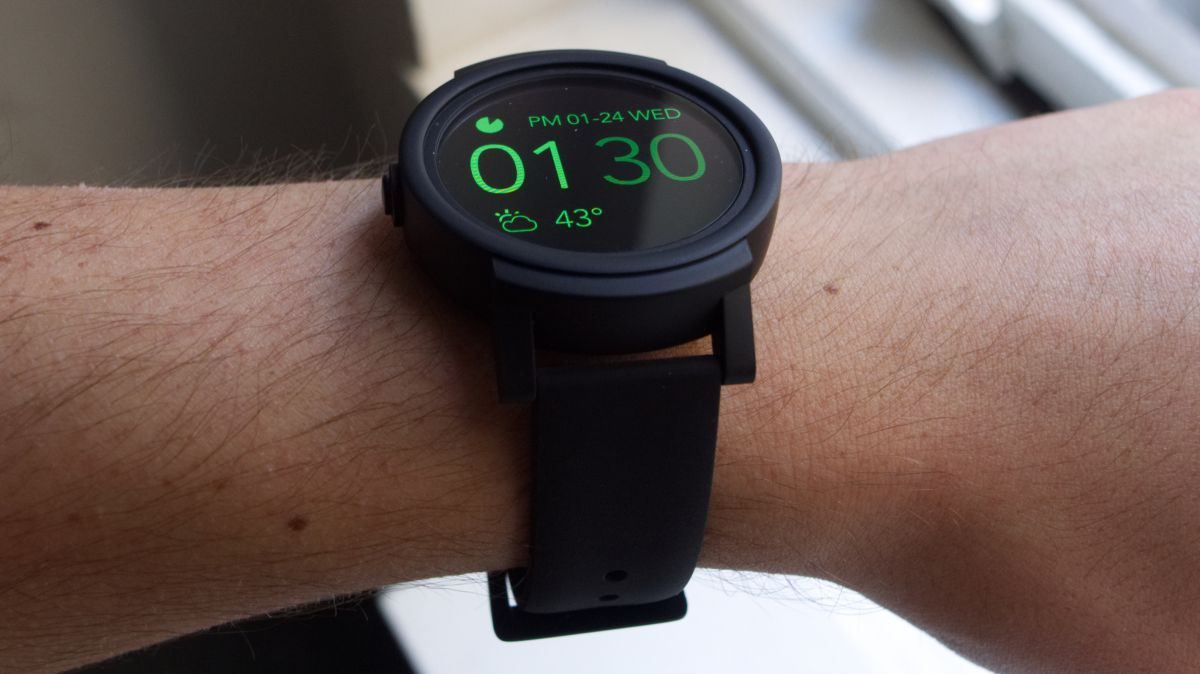
\includegraphics[width=1\textwidth]{ticwatche.jpg}
    \caption{\textit{Ticwatch E} versión negra.}
    \label{fig:ticwatch}
\end{figure}

Entre sus características técnicas, cabe destacar que es un dispositivo con un procesador de doble núcleo a 1.2 GHz, MTK MT2601, basado en ARM Cortex-A7. Esto implica que es un procesador de bajo consumo y potencia moderada. La memoria RAM es de 512 MB y la memoria ROM son 4 GB. Para el GPS admite varios sistemas, GPS, GLONASS y Beidou. GLONASS es el GPS de Rusia y Beidou el de China. Tiene Bluetooth 4.1 BLE, que está especializado para aplicaciones al Internet of Things (IoT) por su bajo consumo. Respecto al resto de sensores, posee acelerómetro, giroscopio, sensor de proximidad, brújula electrónica y monitor del pulso.

\section{Software}

\subsection{Android Studio}

\textit{Android Studio} es el IDE (\textit{Integrated Development Environment}\footnote{Entorno de desarrollo integrado}) que recomienda Google para desarrollar aplicaciones destinadas a dispositivos basados en Android. Está desarrollado por IntelliJ, y es similar a sus otros productos como pueden ser Idea (Java), Pycharm (Python), PHPstorm (PHP). La interfaz es intuitiva y muy completa.

En este caso, para programar ambas cosas, hay que crear un proyecto adecuado para ello. En la pantalla inicial hay que seleccionar una versión objetivo, y el dispositivo para el que está desarrollado. La versión mínima con la que  se quiera desarrollar limita el mercado máximo de la aplicación, por la compatibilidad. Es decir, si elegimos como versión mínima la Android 6.0 (\textit{Marshmallow}), todos los dispositivos con la versión 6.0 o superior podrían acceder a la aplicación. Android 6.0 es una buena versión mínima, ya que se introdujeron grandes cambios, sobretodo a la hora de los permisos que requieren las aplicaciones, que los pide individualmente al usuario, al contrario que en versiones previas, que se aceptaban todos los permisos a la hora de instalar. Esto lo acercó más al sistema que tiene iOS, en el que los permisos se eligen individualmente y pueden ser cancelados desde las opciones de la aplicación. Elegir esta versión ofrece entorno al 65\% de los dispositivos Android como mercado (compatibles), y esta cifra irá aumentando conforme los teléfonos antiguos salgan del mercado.

También, la elección de esta versión tiene otras razones. No es una versión excesivamente antigua, por lo que el estilo de programación se mantiene más o menos igual. Esto es importante porque Android es un sistema que cambia a menudo, provocando que fragmentos de código perfectamente funcional pase a estar \textit{deprecated}, es decir, anticuado.

En el \textit{smartwatch}, la versión mínima ha de coincidir con la del teléfono, pero es menos importante, ya que aunque Google actualice todos sus dispositivos a la vez, y haga un Android 7.0 para \textit{smartphones} y para \textit{smartwatches}, los cambios son más livianos en el sistema operativo de los relojes inteligentes.


\subsection{Matlab}

Matlab (\textit{Matrix Laboratory}) es un idioma de programación orientado a cálculos matemáticos y especializado en cálculo con matrices, de forma nativa. En Matlab no existen arrays, existen matrices de una columna o una fila, no existen variables, existen matrices 1x1. Esto hace que para el tratamiento de grandes volúmenes de datos sea una herramienta muy potente donde otros idiomas cojean. Matlab fue creado en los 70 para evitar tener que usar Fortran, en la universidad de Nuevo México. Rápidamente se extendió en el ambiente académico y a partir de 1984 se unieron sus creadores para comercializarlo. 

Matlab es muy sencillo, y se obtienen resultados de manera muy rápida. El problema es la compatibilidad. Las redes neuronales desarrolladas en Matlab no pueden ser exportadas a otros sistemas de forma sencilla, y normalmente, en dispositivos móviles no es eficiente, ya que no es un idioma de programación pensado para ellos.

Que Matlab sea un lenguaje muy sencillo lo hace muy indicado para introducir el problema y ver si la hipótesis está bien encaminada. Por eso, ha sido muy útil para comprobar en la fase temprana de desarrollo de este proyecto que una red neuronal podía llevar a cabo el trabajo, si sería eficiente y el tipo básico de red que se requería. En esos tres objetivos Matlab fue una herramienta muy potente, pero desgraciadamente, los problemas mencionados anteriormente con Android hicieron que otro tipo de herramientas fuera necesaria.

\subsection{TensorFlow}

Tensorflow es un paquete(o un \textit{framework}) de Python \textit{open source}, centrado en aplicaciones de inteligencia artificial. Es el programa más conocido y utilizado para este tipo de aplicaciones. La comunidad es bastante grande por lo que hay recursos de ayuda, además de una gran API (\textit{Application Programming Interface}), la documentación oficial.

El problema de este tipo de programas \textit{open source} es la compatibilidad con el hardware, que no es siempre la mejor y que la comunidad se fragmenta debido a ello. Las incompatibilidades de nuevas versiones o diversas otras razones como mantener el \textit{status quo} en una aplicación que ya funciona. Esto provoca que los recursos en la red no siempre sean los correctos para la versión que se está usando.

Esto hizo que durante el desarrollo del algoritmo de este trabajo se usaran diferentes versiones de TensorFlow hasta que se consiguió finalmente la correcta. En este caso, se utilizó la versión más actualizada, \textit{2.0 alpha}, debido a que los recursos oficiales, siempre actualizados, son los más fiables, y como se mencionó anteriormente, tienen una gran documentación, con ejemplos ilustrativos y explicaciones de las funciones que se pueden utilizar.

Además, una gran ventaja que tiene TensorFlow frente a otros paquetes similares es su implementación en Android. TensorFlow nació inicialmente como un proyecto interno de Google para tener una herramienta para implementar algoritmos de inteligencia artificial. Esto facilitó que creara una librería para Android que pudiera aplicar estas soluciones en aplicaciones ligeras.


 
\section{Red Neuronal}

La red neuronal es también una herramienta y una parte fundamental de este trabajo. La red ha sido desarrollada en Python, usando TensorFlow, y dentro de éste, se ha utilizado Keras. Keras es, simplemente, una interfaz de trabajo que hace más sencillo TensorFlow. Permite usar las herramientas de TensorFlow pero a un nivel mucho superior a este. Hace la sintaxis de programación más sencilla que con TensorFlow puro.

Si nos fijamos en la estructura interna, es un Perceptrón Multicapa con 4 capas contando la de entrada y salida, 2 de ellas internas por tanto. En la figura \ref{fig:redneuronal} se puede ver un diagrama de mi red neuronal.
\begin{figure}[h]
    \centering
    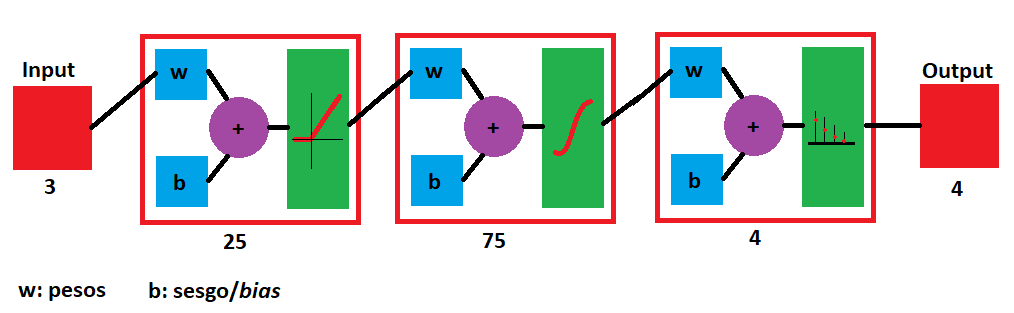
\includegraphics[width=1\textwidth]{miredneuronal.png}
    \caption{Red Neuronal.}
    \label{fig:redneuronal}
\end{figure}

Donde se ve que la primera capa, que es la de entrada, al no tener función de activación, solo es una red que recibe los datos de entrada de tres dimensiones, los ejes X, Y y Z del acelerómetro. La primera capa interna, de 25 neuronas, tiene función de activación \textit{reLU}, que es una función rectificadora. La siguiente capa, de 75 neuronas tiene función de activación sigmoide, y finalmente la cuarta capa, de salida, tiene una función de activación \textit{softmax}. Finalmente de ahí salen las salidas, que son las cuatro clases de movimiento que se quieren detectar, reposo, andando, corriendo y las caídas.

La elección del número de capas, número de neuronas y la función de activación de cada capa ha sido un proceso largo de prueba y error. Esto se debe sobretodo a dos problemas que tienen las redes: \textit{Overfitting} y \textit{Underfitting}. El primero, mas sencillo de comprender, es el proceso por el cual una red neuronal no es capaz de alcanzar valores altos de acierto, ni en los datos de entrenamiento ni en los datos de validación. Este problema se soluciona normalmente añadiendo neuronas, capas o aumentando el número de periodos de entrenamiento, es decir, aumentando la potencia bruta de la red. En la figura \ref{fig:underfit} se puede observar este efecto claramente.

\begin{figure}[h]
    \centering
    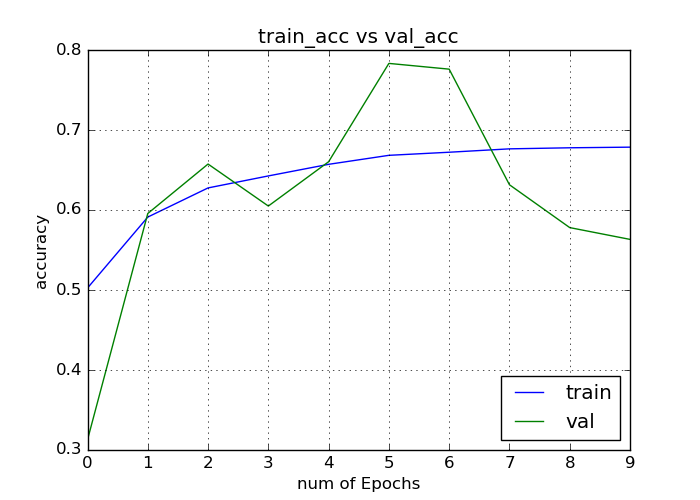
\includegraphics[scale=0.7]{underfit.png}
    \caption{Caso de \textit{underfit}.}
    \label{fig:underfit}
\end{figure}

El otro caso es algo más difícil de explicar. Ocurre cuando la red neuronal tiene tanta potencia que es capaz de aprenderse una mayoría de datos de entrenamiento. Esto hace que en apariencia la red esté funcionando muy bien, pero al introducir los datos de validación, se ve que la red no ha aprendido los patrones de clasificación. Esto se evita de varias formas, reduciendo la potencia bruta de la red, al contrario que en el caso anterior, pero también aumentar el número de datos de entrenamiento puede solucionarlo. En la figura \ref{fig:overfit} se puede observar este defecto del algoritmo.

\begin{figure}[h]
    \centering
    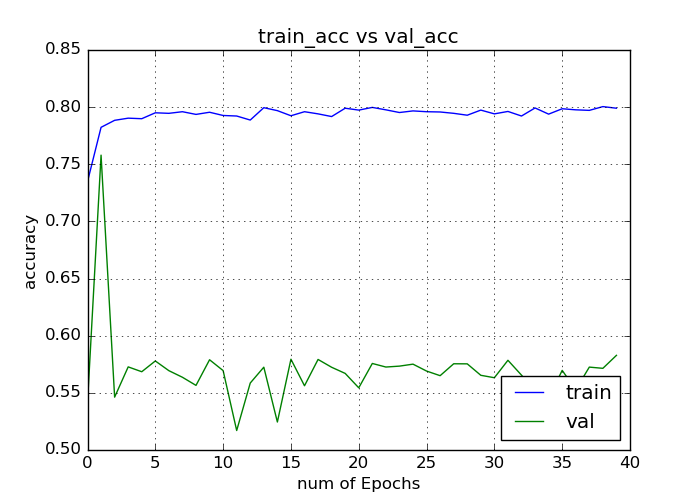
\includegraphics[scale=0.7]{overfit.png}
    \caption{Caso de \textit{overfit}.}
    \label{fig:overfit}
\end{figure}

Pero estos no son los dos únicos errores a los que acostumbran las redes neuronales. A veces tienen comportamientos erráticos, de repente aprenden de golpe o incluso olvidan. En estos casos, lo más normal es que con un pequeño cambio la red se reajuste sola. Esto puede ser debido a que la red se quede aprendiendo en torno a un mínimo, pero que no sea el mínimo absoluto, por lo que no se obtiene un resultado válido.


\chapter{Metodología}
En este capítulo se va a describir la metodología para la obtención de los resultados de la parte experimental del trabajo. Esta metodología se ha estructurado en tres fases. En primer lugar, la toma de datos, por el \textit{smartwatch}. Posteriormente estos datos han de ser enviados al \textit{smartphone}. Finalmente, estos datos en el \textit{smartphone} son clasificados por la inteligencia artificial aplicada. Se procederá a continuación a detallar el proceso.

\section{Toma de datos}

Para la toma de datos se ha usado una aplicación creada para este propósito. Esta aplicación cuenta con una versión para Android para el \textit{smartphone} y otra versión para Android Wear en el \textit{smartwatch}.

Como puede verse en la figura \ref{fig:mesh2}, la interfaz de esta aplicación experimental es simple, donde se ha priorizado la funcionalidad ante todo.

\begin{figure}[h]
    \centering
    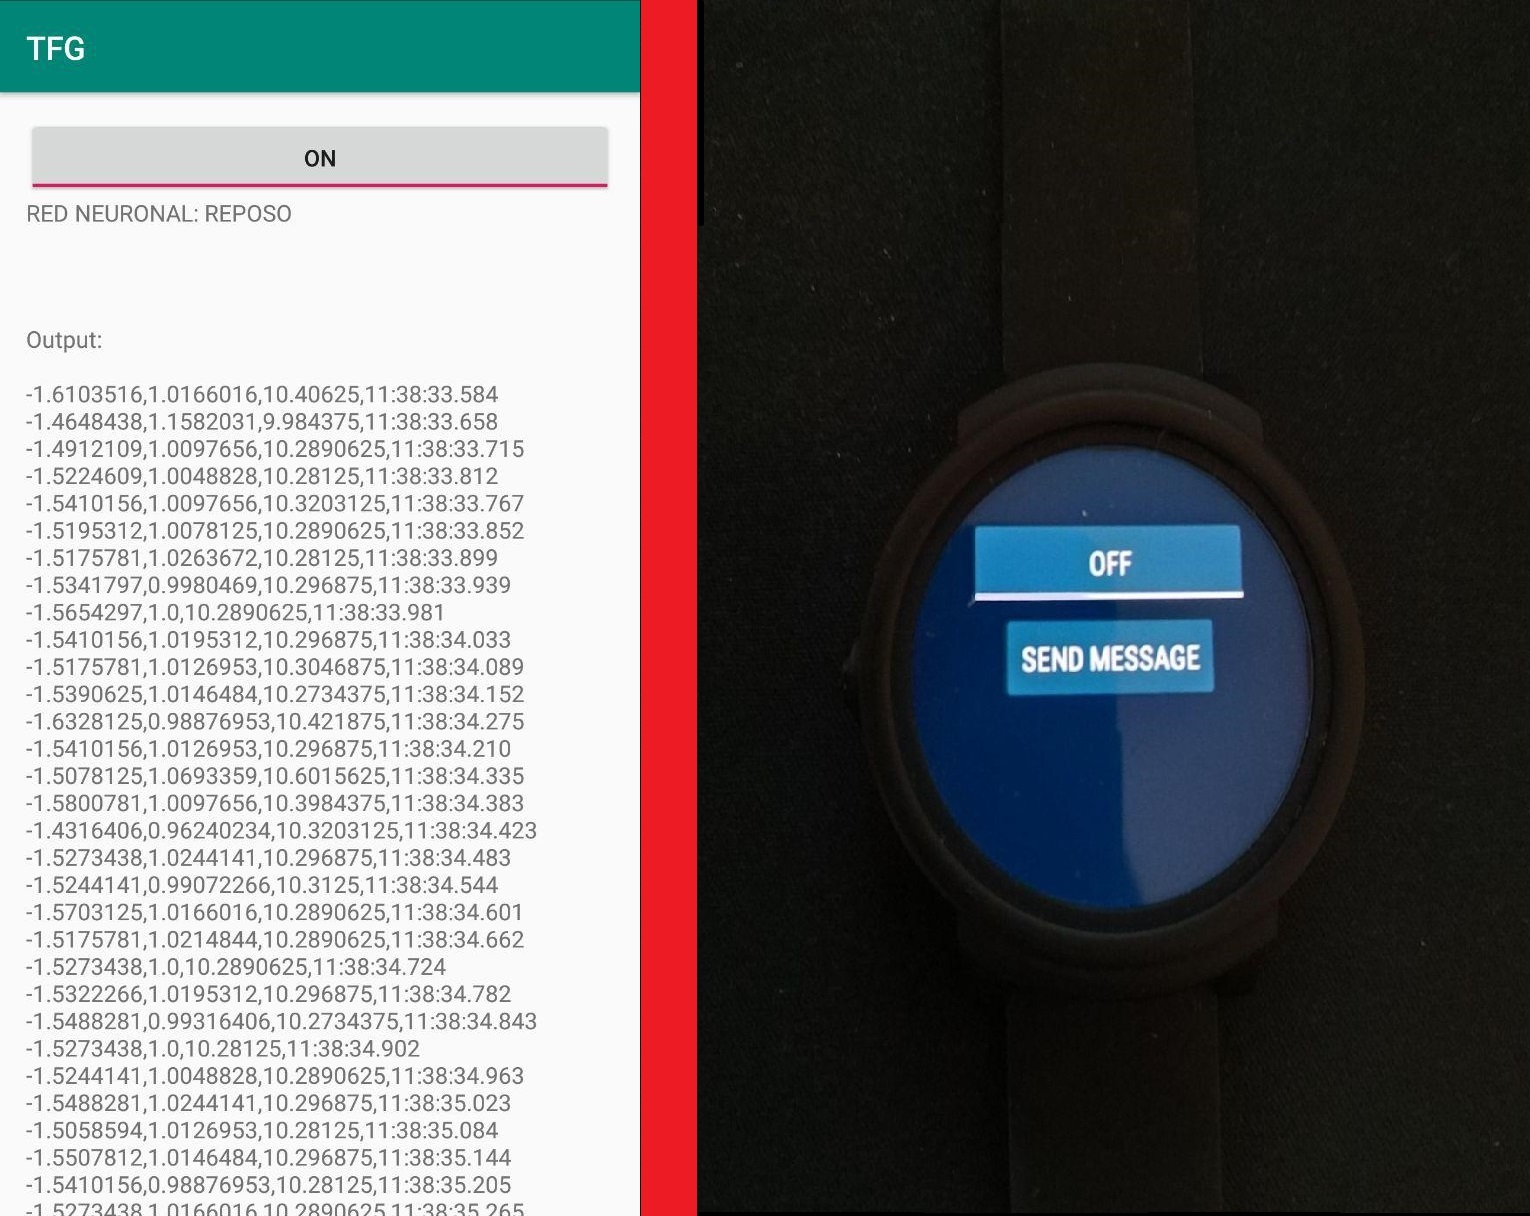
\includegraphics[width=0.8\textwidth]{Interfaces.jpg}
    \caption{Interfaz del \textit{smartphone} (izquierda) y \textit{smartwatch} (derecha).}
    \label{fig:mesh2}
\end{figure}

En la figura \ref{fig:mesh2}, a la izquierda está la aplicación en el \textit{smartphone} y a la derecha la del \textit{smartwatch}. La del móvil tiene un botón para activar el recibir mensajes, una sección donde se muestra lo que detecta la red neuronal y un espacio donde se muestran los últimos mensajes recibidos. Esta lista se va actualizando a tiempo real conforme se reciben los datos al igual que la predicción de la red. Por otro lado, la del \textit{smartwatch} tiene dos botones. El superior es un botón pulsador (\textit{on/off}), un interruptor, y es el encargado de mandar los datos de los sensores al \textit{smartphone}, mientras que el botón de abajo, \textit{SEND MESSAGE}, es un botón de comprobación, cuyo propósito es verificar que se manden los mensajes bien a la aplicación del \textit{smartphone}

Una vez expuestas las interfaces de trabajo de la aplicación, se mostrará en una tabla la metodología seguida para tomar los datos de entrenamiento (ejemplo) para la red neuronal.

\begin{table}[h]
\centering
\caption{Metodología toma de datos}
\begin{tabular}{| c | c |}
\hline
Reposo & Toma de datos sentado y de pie. \\
\hline
Andando & Recorrido fijo. \\
\hline
Corriendo & Recorrido fijo. \\
\hline
Cayendo & Proceso de pruebas por repetición \\
\hline
\end{tabular}
\label{tabla1}
\end{table}

La toma de datos se hizo en un recorrido fijo de circuito cerrado. Las medidas de las caídas fueron tomadas en distintas posiciones y direcciones.

\newpage
\section{Análisis de los datos}

A continuación se van a mostrar los datos obtenidos, analizando en primer lugar las características generales de estos datos que aparecen representadas en la Tabla \ref{tabla2}.
\begin{table}[h]
\centering
\caption{Datos generales}
\begin{tabular}{| c | c | c | c |}
\hline
 & Eje X & Eje Y & Eje Z \\
\hline
Muestras & 19337 & 19337 & 19337 \\
\hline
Media & -3.036879 & -3.869599 & 4.779501 \\
\hline
Desv. Típica & 7.213168 & 8.843972 & 6.318493 \\
\hline
Mínimo & -78.437500 & -78.437500 & -57.375000 \\
\hline
Máximo & 72.937500 & 78.437500 & 78.437500 \\
\hline
\end{tabular}
\label{tabla2}
\end{table}

Se pueden observar varios aspectos de interés. Lo primero es que los valores mínimo y máximo coinciden en valor absoluto en 4 de 6 casos posibles, lo cual nos hace intuir que el valor máximo de medida del acelerómetro es ese. Esto podría ser un problema, pero en este caso, la media en los tres ejes está en [-4, 5] y la desviación típica es menor a 10 en todos casos, por lo que la mayoría de los puntos medidos están lejos de esos valores máximos de corte.  A ese valor máximo se le llamará aceleración de corte.

Los datos miden directamente la aceleración sufrida en $m s^{-2}$. La frecuencia de recogida de datos es de 17 Hz, es decir, 17 medidas por segundo. En las gráficas de las paginas posteriores, el eje Y corresponde a la aceleración medida, y el de abscisas al número de muestra.

Con esta frecuencia de recogida nos aseguramos de que ningún evento de los que se quieren medir va a ocurrir en un intervalo entre dos medidas, es decir, que no se detectara. En nuestro caso implica que no se podrían medir sin perdidas eventos que duren 1/17 s o más. Si el tiempo de reacción media de un humano es de 0.15 segundos, y cayendo es evidente en la experiencia que nos da tiempo a reaccionar y colocar las manos o al menos intentar evitar mayores daños, se entiende que la caída dura más, por lo que tiene una frecuencia mayor a 1/17 Hz, y por tanto, el evento más rápido de los que medimos tiene una duración mayor a la necesaria, y el resto duran más que las caídas por lo que se pueden detectar. 

\subsection{Reposo}

A continuación se muestra el resumen de los datos en la tabla \ref{tabla3}.

\begin{table}[h]
\centering
\caption{Datos Reposo}
\begin{tabular}{| c | c | c | c |}
\hline
 & Eje X & Eje Y & Eje Z \\
\hline
Muestras & 5356 & 5356 & 5356 \\
\hline
Media & -0.091385 & -0.363739 & 10.359101 \\
\hline
Desv. Típica & 0.037410 & 0.026726 & 0.023491 \\
\hline
Mínimo & -0.926270 & -0.619629 & 10.007812 \\
\hline
Máximo & 0.605469 & 0.385254 & 11.187500 \\
\hline
\end{tabular}
\label{tabla3}
\end{table}

Como es lógico, en estos datos la desviación típica es muy baja, lo que indica que los datos no están dispersos. Esto es así porque en los datos en reposo no ha habido movimientos y por tanto el acelerómetro ha estado mandado datos similares. Es por otro lado lógico que en el eje Z detecte en torno a 10, ya que ese es el valor aproximado de la aceleración gravitatoria terrestre.

\begin{figure}[h]
    \centering
    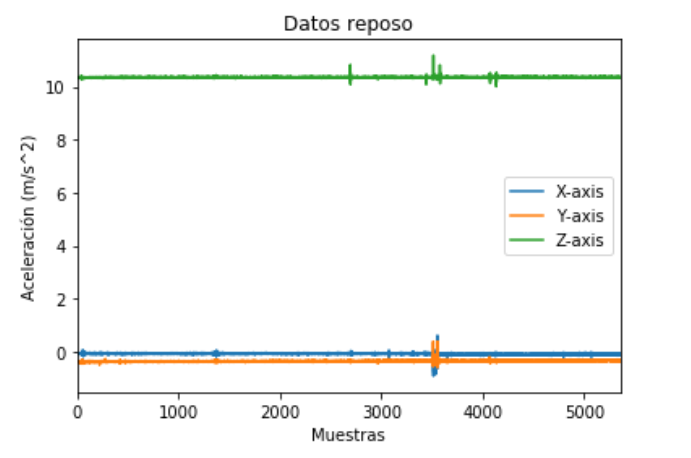
\includegraphics[width=0.6\textwidth]{reposodatos.png}
    \caption{Datos representados de reposo.}
    \label{fig:reposodatos}
\end{figure}

En la gráfica de los datos de la figura \ref{fig:reposodatos} se puede observar que los datos son estables salvo pequeños movimientos. El eje de ordenadas representa la aceleración en $m s^{-2}$ sufrida y el eje de abscisas es simplemente el número del muestra.

\newpage
\subsection{Andando}

Ahora los datos andando, en la tabla \ref{tabla4}.

\begin{table}[h]
\centering
\caption{Datos Andando}
\begin{tabular}{| c | c | c | c |}
\hline
 & Eje X & Eje Y & Eje Z \\
\hline
Muestras & 4815 & 4815 & 4815 \\
\hline
Media & -9.978337 & -2.977451 & 0.679224 \\
\hline
Desv. Típica & 3.550272 & 1.980726 & 1.415865 \\
\hline
Mínimo & -25.953125 & -16.734375 & -6.371094 \\
\hline
Máximo & 11.601562 & 8.281250 & 14.507812 \\
\hline
\end{tabular}
\label{tabla4}
\end{table}

Como se puede observar, ahora la desviación típica es mucho mayor, lo que implica una mayor rango de valores de los datos. También se puede ver que en ningún momento el valor de los máximos o mínimos coincide con los valores de la \ref{tabla2}, por lo que todos los datos de andando están por debajo de la aceleración de corte.

\begin{figure}[h]
    \centering
    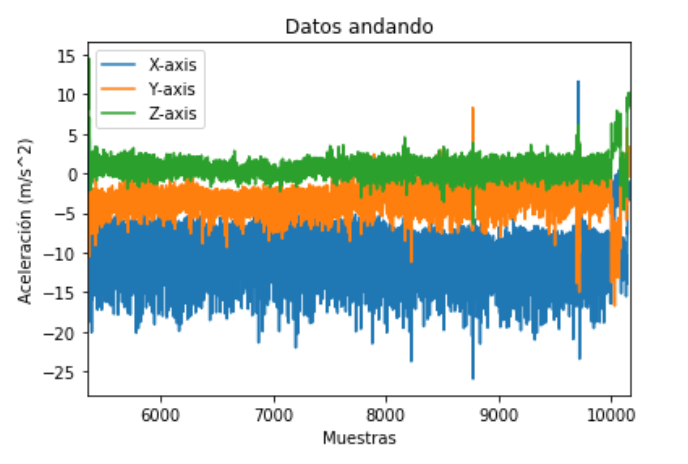
\includegraphics[width=0.6\textwidth]{andandodatos.png}
    \caption{Datos representados andando.}
    \label{fig:andandodatos}
\end{figure}

En la gráfica en la figura \ref{tabla5} se observan los resultados deducidos de la tabla \ref{tabla4}, mayor desviación sin llegar a valores demasiado altos de aceleración.

\newpage
\subsection{Corriendo}

\begin{table}[h]
\centering
\caption{Datos Corriendo}
\begin{tabular}{| c | c | c | c |}
\hline
 & Eje X & Eje Y & Eje Z \\
\hline
Muestras & 4981 & 4981 & 4981 \\
\hline
Media & -0.632807 & -11.085089 & 1.323010 \\
\hline
Desv. Típica & 7.645861 & 12.869971 & 3.306390 \\
\hline
Mínimo & -34.000000 & -64.437500 & -19.078125 \\
\hline
Máximo & 36.156250 & 14.281250 & 23.859375 \\
\hline
\end{tabular}
\label{tabla5}
\end{table}

En este caso vemos que la desviación típica vuelve a crecer, lo que es esperado, ya que al correr se hacen movimientos más bruscos que andando y en reposo. Al igual que antes, no se llega a la aceleración de corte, por lo que ningún dato corriendo va a perder precisión.

\begin{figure}[h]
    \centering
    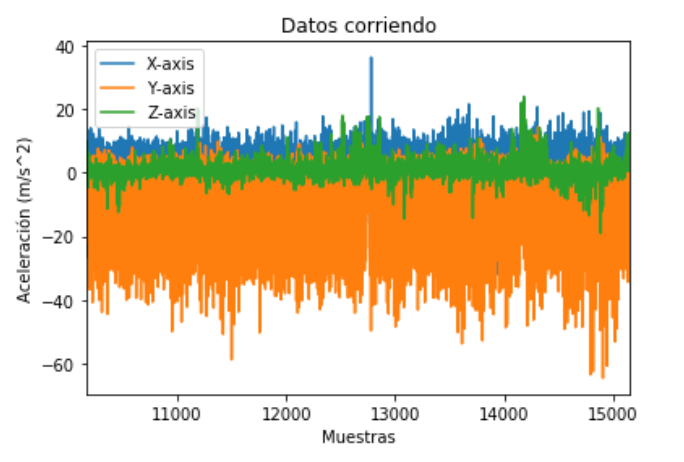
\includegraphics[width=0.5\textwidth]{corriendodatos.png}
    \caption{Datos representados corriendo.}
    \label{fig:corriendodatos}
\end{figure}

Como se puede observar, ahora ya si hay mayor desviación de los datos en la gráfica, sobretodo en el eje Y.

\subsection{Cayendo}

Finalmente los datos cayendo en la tabla \ref{tabla6}.

\begin{table}[h]
\centering
\caption{Datos Corriendo}
\begin{tabular}{| c | c | c | c |}
\hline
 & Eje X & Eje Y & Eje Z \\
\hline
Muestras & 4185 & 4185 & 4185 \\
\hline
Media & -1.681473 & -0.794982 & 6.470128 \\
\hline
Desv. Típica & 9.005075 & 8.468682 & 9.638507 \\
\hline
Mínimo & -78.437500 & -78.437500 & -57.375000 \\
\hline
Máximo & 72.937500 & 78.437500 & 78.437500 \\
\hline
\end{tabular}
\label{tabla6}
\end{table}

En este caso podemos ver que los datos, por lo que a la desviación típica respecta, no están más dispersos que los de la sección anterior, sin embargo, se puede observar que los valores mínimos y máximos en valor absoluto son iguales en muchos casos, lo que implica que se llega a la aceleración de corte.

\begin{figure}[h]
    \centering
    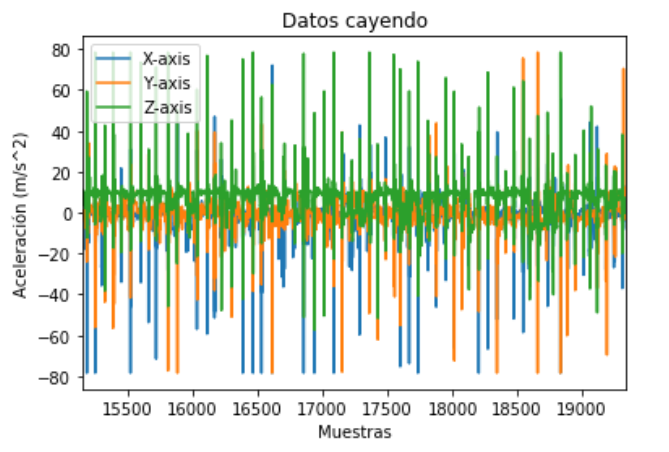
\includegraphics[width=0.6\textwidth]{cayendodatos.png}
    \caption{Datos cayendo.}
    \label{fig:cayendodatos}
\end{figure}

Como se puede observar en la figura \ref{fig:cayendodatos}, ahora se muestra una gráfica con grandes picos en todas direcciones, lo que tiene sentido ya que en las caídas es donde mayor aceleración hay de estos cuatro tipos de movimientos.


\subsection{Comentarios de los datos}

Pudiera parecer que se podrían identificar los datos con algún tipo de algoritmo tradicional, en el que se vea que si hay un pico muy grande de aceleración entienda que es una caída, y que en los casos de reposo también pudiera acotarse unos límites para identificar el movimiento. Entre correr y andar sería más difícil, habría que hacer algún algoritmo bastante complejo pero la opción existe. Desgraciadamente, Android es un lenguaje basado en Java, con todo lo que ello implica. Las limitaciones a la hora de los cálculos son evidentes, y un algoritmo así requeriría recibirlo del \textit{smartwatch}, aplicarle algoritmos de transformadas de Fourier en tiempo real, cálculos matemáticos constantes para la identificación del movimiento y actualizarlo en pantalla. Esta carga para el procesador haría que la batería durara muy poco, por lo que esa opción no es viable.

En cambio, una red neuronal entrenada no consume apenas recursos, los pesos se cargan, la red un dato y elige un resultado en función del entrenamiento previo. Hay que remarcar que una red neuronal, desde el proceso de entrenamiento hasta el de validación es un proceso largo y que lleva un tiempo de computación notable, pero una vez pasado ese proceso, el proceso de selección con datos es muy rápido. Esa es una de las grandes ventajas de las redes neuronales en este caso. Además, TensorFlow Lite, la librería para Android, es muy eficiente.

No solo es la ventaja de la velocidad de computación, sino que además, el código en el caso de la red neuronal es mucho más compatible y expansible. Solo requiere de la toma de datos de entrenamiento y volver a reentrenar la red. Sin embargo, en el caso de un algoritmo tradicional, en el caso de querer añadir un movimiento más, habría que hacer unas reglas de selección y de identificación mucho más estrictas, haciendo el código mucho más complejo por solo un elemento más. 

Todo esto, junto a que el funcionamiento superior por parte de la vía algorítmica no está asegurado se opta en este trabajo por la red neuronal. Pero no es la única opción. En la bibliografía se encuentran ejemplos de la vía algorítmica\cite{s150818901}, por lo que tampoco es una opción imposible.


\section{Programación}

Para extraer los datos, se han usado las herramientas de Android. Esto simplifica mucho el trabajo ya que no hay necesidad programar una interfaz completa de comunicación, vale con la incluida en Android, conocida como \textit{Data Layer}. Es una capa de datos que se sincroniza entre todas las instancias del programa. Esto quiere decir que si la aplicación desde el módulo del \textit{smartwatch} manda un dato a esta capa, la aplicación desde el \textit{smartphone} tiene acceso a esos datos. Así, la comunicación es mucho más sencilla.

Hay que programar el acceso a la data layer para escribir y para leer. Para ello, primero tenemos que encontrar los nodos conectados. Cada instancia de la aplicación en cada dispositivo es un nodo, en nuestro caso hay dos nodos, el del \textit{smartwatch} y el del \textit{smartphone}. La forma más sencilla es crear un servicio en cada nodo que se encarga automáticamente de recibir y mandar mensajes. Así, con un pequeño fragmento de código se está comprobando constantemente si hay datos nuevos y si están en el sitio que nos interesa. Hay que definir un camino (ruta) donde van a estar los datos, en el código se llama \textit{message\_path}. Si está en el lugar adecuado, entonces ese mensaje se manda a la actividad principal y se muestra en pantalla.

Por otro lado, en el tratamiento de datos, se utiliza el \textit{interpreter} de TFlite, el paquete de TensorFlow pensado para Android. Para usarlo, se ha de añadir el archivo donde se guarda la red neuronal en la carpeta de \textit{assets} del proyecto. Una vez ahí, solo hay que hacer las llamadas con un dato de entrada válido y un vector de salida.

Cuando esto ocurre, el \textit{interpreter} devuelve un vector de salida, donde se muestra la probabilidad que le otorga la red neuronal a cada clase. Esto se aprovecha para ir haciendo la suma de varias mediciones para obtener un resultado mejor. En este caso, se ha elegido acumular ocho medidas, ya que se entiende que ese arco de alrededor de medio segundo ofrece una ventana de información adecuada para detectar los movimientos. Es lo suficientemente corto como para responder rápido a los cambios del usuario y aumenta la precisión del resultado al promediar entre varias medidas.

Finalmente, esta predicción de la actividad detectada tras ocho medidas (aproximadamente medio segundo) se muestra en pantalla. Además, puede ser guardada en un archivo de texto para ser analizados con mayor detalle posteriormente.

\newpage
\chapter{Resultados}

A continuación se mostrarán y explicarán los resultados obtenidos en diversas fases del proyecto. Primero, se procederá con los obtenidos en Python, en el entrenamiento de la red neuronal. Posteriormente se mostrarán los obtenidos en Android.

Primero se procederá con los datos de entrenamiento de la red neuronal. A continuación en la figura \ref{fig:possibleBF}, se muestra la precisión del entrenamiento frente a la precisión de validación. En este caso, la precisión mide el número de muestras acertadas por la red neuronal entre las totales. En el eje de ordenadas se observa la precisión total. En el de abscisas el número de eras por el que pasa la red neuronal. Se considera una era cada vez que la red clasifica todos los datos.

\begin{figure}[h]
    \centering
    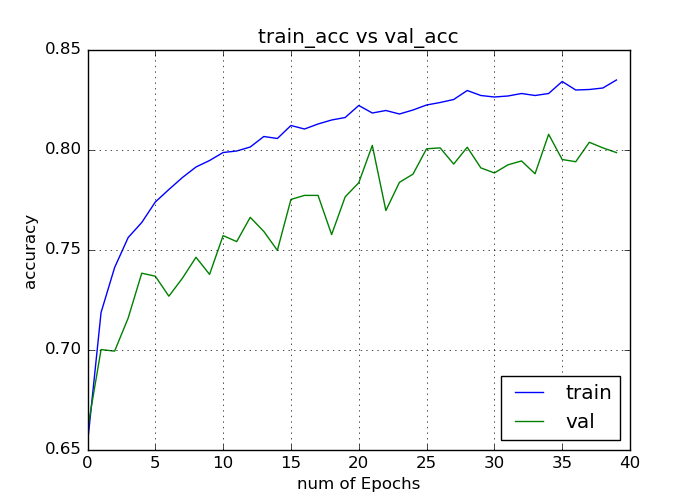
\includegraphics[width=0.8\textwidth]{PossibleBF_2.png}
    \caption{Resultado del entrenamiento.}
    \label{fig:possibleBF}
\end{figure}

\newpage
Se puede observar que la precisión de validación es menor que la precisión de los datos de entrenamiento, algo lógico, ya que la red se está entrenando en base a ellos, pero no es preocupante ni estamos ante un caso de \textit{overfit} como el de la figura \ref{fig:overfit}, ya que la precisión de los datos de validación sigue aumentando y la diferencia de precisión no es muy alta, menos del 3\%. Los datos finales son de una precisión del 81\% a nivel de red neuronal y posteriormente en Android aumenta más.

Para un estudio más en profundidad de los datos existe lo que se denomina comúnmente una matriz de confusión, que es una forma gráfica de ver los resultados de la red y donde se encuentran los errores.

La tabla \ref{confusionTraining} muestran la matriz de confusión de los datos de entrenamiento. Las columnas muestra los datos de la clase y la clasificación que ha hecho la red neuronal. Por tanto, la primera columna, los datos en reposo, de los 4632 datos que había, la red neuronal ha clasificado 4101 como reposo, 10 como andando, 9 como corriendo y 512 como cayendo. Esto hace una precisión del 89\%, como se muestra en la última fila. Por otro lado, las filas de datos muestran todos los datos clasificados como cada clase. Por ejemplo, la segunda fila, de andando, muestra que la red ha clasificado correctamente 3490 datos y erroneamente en forma de falsos positivos los 321 restantes, y el porcentaje de datos correctos entre la suma de los correctos y los falsos positivos se muestra en la última columna.


\begin{table}[h]
\centering
\begin{tabular} {| c || c | c | c | c || c |}
  \hline
   & Reposo & Andando & Corriendo & Caídas & \% $\frac{aciertos}{aciertos + falsos \, positivos}$\\
  \hline
  \hline
  Reposo & \cellcolor{green!25}4101 & 0 & 0 & 0 & 100\% \\
  \hline
  Andando & 10 & \cellcolor{green!25}3490 & 277 & 34 & 92\% \\
  \hline
  Corriendo & 9 & 933 & \cellcolor{green!25}2840 & 195 & 71\% \\
  \hline
  Cayendo & 512 & 282 & 832 & \cellcolor{green!25}1806 & 52\% \\
  \hline
  \hline
  \% aciertos red & 89\% & 74\% & 72\% & 89\% & \\
  \hline
\end{tabular}
\caption{Matriz de confusión de los datos de entrenamiento.}
\label{confusionTraining}
\end{table}

En la tabla \ref{confusionValidation} se puede ver la matriz de confusión de los datos de validación. Los datos coinciden en mayor o menor medida a los de entrenamiento, siendo estos datos de validación medidas que la red nunca había visto, por lo que son independientes y examinan que el entrenamiento funciona.

\begin{table}[h]
\centering
  \begin{tabular} {| c || c | c | c | c || c |}
  \hline
   & Reposo & Andando & Corriendo & Caídas & \% $\frac{aciertos}{aciertos + falsos \, positivos}$\\
  \hline
  \hline
  Reposo & \cellcolor{green!25}1250 & 0 & 0 & 0 & 100\% \\
  \hline
  Andando & 0 & \cellcolor{green!25}929 & 71 & 0 & 93\% \\
  \hline
  Corriendo & 7 & 196 & \cellcolor{green!25}742 & 55 & 74\% \\
  \hline
  Caída & 87 & 77 & 183 & \cellcolor{green!25}403 & 54\% \\
  \hline
  \hline
  \% aciertos red & 93\% & 77\% & 74\% & 88\% & \\
  \hline
  \end{tabular}
    \caption{Matriz de confusión de los datos de validación.}
  \label{confusionValidation}
\end{table}

\newpage
De estas tablas se puede sacar mucha información interesante. Quizá la más llamativa sea el número de falsos positivos entre los datos de caída. Esto podría ser un grave problema para el funcionamiento de una aplicación. Sin embargo, al promediar los datos de ocho medidas en la aplicación este efecto disminuye notablemente. Además, como las caídas eran el único patrón que se podía obtener de forma determinista de forma clara, se le han añadido a la detección para dar más peso a las caídas. 


\begin{figure}[h]
    \centering
    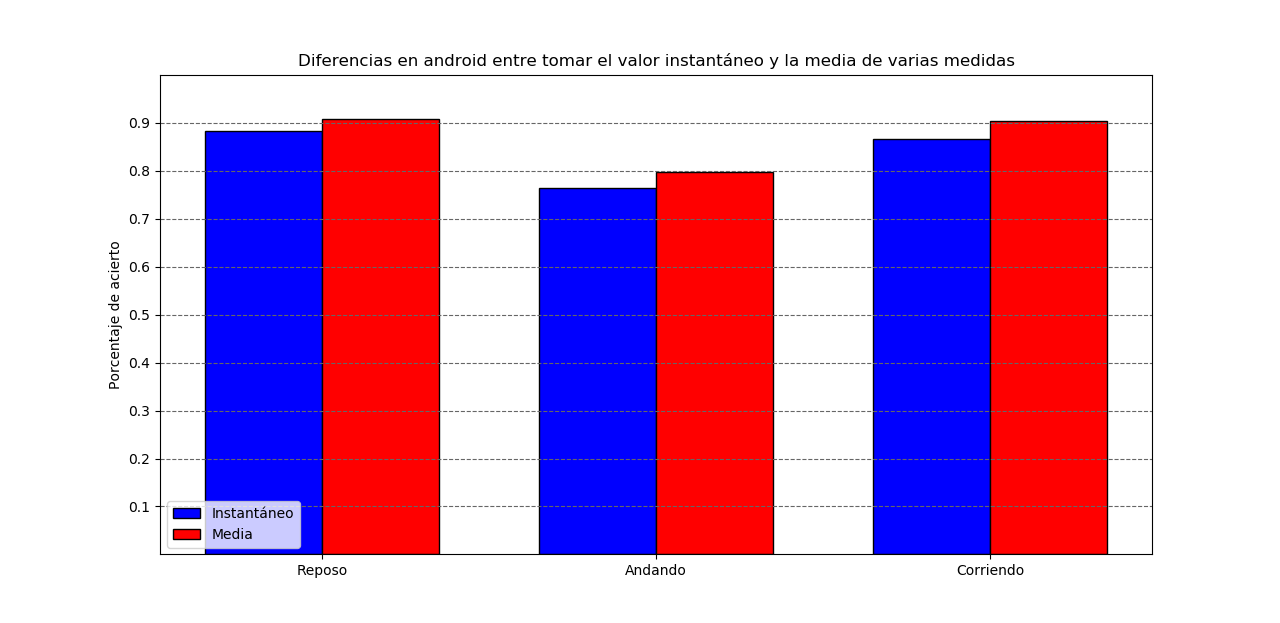
\includegraphics[width=0.8\textwidth]{finalesAndroid.png}
    \caption{Resultados en Android.}
    \label{fig:finalesAndroid}
\end{figure}

En la figura \ref{fig:finalesAndroid} se encuentran los resultados obtenidos en Android. Se puede observar en las clases reposo, andando y corriendo sus resultados instantáneos frente a los resultados obtenidos al decidir tras acumular ocho datos. Como se puede ver, no hay mucha diferencia, lo que indica que la red funciona bien incluso con una sola entrada, pero aún así es notable. Se han omitido los datos de caída ya que se ha visto que las detecta con una precisión del 90\% (27 de 30). Esto es así debido al código, en el que se ha añadido cierto peso a la medida del acelerómetro si detecta un movimiento muy brusco. Se considera detección de una caída como que la red detecte al menos durante un periodo de medio segundo la caída en un periodo menor a un segundo, es decir, que en las próximas dos medidas detecte la caída. Esto es suficiente como para poder lanzar una alarma en el caso en el que la detecte, por lo que se obtiene un resultado final importante, se podría automatizar el aviso a emergencias si se detecta una caída y el usuario no responde.

\newpage
\chapter{Conclusiones}

Teniendo en cuenta las limitaciones que nos impone Android, y al no poder tomar simultáneamente los datos del acelerómetro y del giroscopio mantiene un funcionamiento aceptable. Una precisión global del 81\% de acierto está bastante bien y muestra la potencia de las redes neuronales y de la inteligencia artificial.

A continuación, unos comentarios sobre el trabajo:

\begin{enumerate}
\item[1.] Ha sido interesante adentrarse en el mundo de la inteligencia artificial, pues así se da uno cuenta del gran campo que hay de investigación. Además, es el momento adecuado, ya existe la potencia de computación para resolver verdaderos problemas. Se ha hecho una introducción al campo muy interesante y además muy legible, fácil de seguir y comprender.

\item[2.] El internet de las cosas sigue adelante aunque últimamente el término esté de capa caída. La potencia de los dispositivos aumenta y cada vez tienen más utilidad. En este caso se ha usado un dispositivo de uso general para algo muy concreto y que podría tener utilidad para muchas personas.

\item[3.] El potencial para el cambio de la vida de personas ancianas y/o en riesgo es alto. Con una inversión mayor se podría crear una aplicación más precisa que ayudaría a millones de personas, y además no es algo caro, ya que los \textit{smartwatch} son asequibles y son cómodos de llevar. Finalmente, muchas personas mayores están acostumbradas a llevar un reloj, así que el tiempo de adaptación sería corto.

\item[4.] El principal problema de los \textit{smartwatches} sigue siendo, no su potencia, sino su batería. La mayor mejora que podrían obtener este tipo de dispositivos sería en ese campo. Hay otras opciones, como por ejemplo usar una pantalla de bajo consumo que no sea LCD. De esta forma, se podrían obtener dispositivos de batería de gran duración. Como se observó en la sección de antecedentes, la conexión a internet y el LCD hacen bastante proporción del gasto. Con un dispositivo con tecnología e-ink se podría reducir muchísimo el gasto.

\item[5.] Como nota personal, ha sido interesante adentrarse en el mundo de la programación y tratamiento de señales a un nivel más allá del necesario para superar la carrera. De esta forma, he aprendido y ampliado mis conocimientos en el campo, y además lo he disfrutado.

\item[6.] Se ha desarrollado este proyecto enteramente basado en \textit{software} libre. Todo esto es reproducible en casa a coste cero. Esto es importante porque muestra que cada vez más, las técnicas de vanguardia en ciencia no están en manos de corporaciones que las puedan limitar por una u otra razón. Además, la comunidad de este tipo de herramientas libres suele ser abierta y activa, por lo que se resuelven las dudas bastante rápidamente.
\end{enumerate}

Como posibles ampliaciones de este trabajo, se proponen varias cosas. Primeramente, la red neuronal es un Perceptrón multicapa, por lo que se podría obtener mejores resultados con una red convolucional. Si ocurriera eso, habría que implementar la librería de TensorFlow completa para Android, ya que TFlite no contiene todas las funciones de este tipo de redes. Esto haría que la precisión aumentase a costa de un pequeño gasto de batería, ya que la librería completa no está tan optimizada.

Otra posible ampliación sería tomar más datos simultáneamente, por ejemplo acelerómetro y giroscopio a la vez. No es posible en \textit{WearOS} actualmente tomarlo a la vez. Se puede tomar salteado pero no se sabe si manda un dato de acelerómetro, uno de giroscopio y así sucesivamente o te manda diez datos seguidos del acelerómetro y luego otros veintiocho del giroscopio, lo que lo hace inviable. Probablemente con un hardware personalizado en este aspecto podría funcionar mejor.

Se podría probar un método determinista para detectar los patrones. El acelerómetro de este dispositivo puede mandar hasta cíen muestras por segundo, lo que hace una imagen más completa. Esto tendría como retos optimización del proceso, ya que tiene muchos más datos que tratar y además tendrá que transformarlos y aplicarles algoritmos de transformada rápida de Fourier.



\nocite{*}
\addcontentsline{toc}{chapter}{Bibliografía}
\bibliography{mybib2}
\bibliographystyle{ieeetr}

\newpage
\begin{appendices}
Todo el código y material utilizado para la realización de este proyecto puede encontrarse en: \emph{https://github.com/Mega259/TrabajoFinGrado}
\end{appendices}

\end{document}


